\PassOptionsToPackage{table}{xcolor}
\documentclass{cernatsnote}
\usepackage[colorinlistoftodos]{todonotes}
\usepackage{placeins}
\usepackage{float}
\usepackage{rotating}
\usepackage{verbatim}
\usepackage{fancyvrb}
\usepackage{listings}
\lstdefinestyle{python}{
  language=Python,
  basicstyle=\small\ttfamily,
  keywordstyle=\color[RGB]{0,0,200}\bfseries,
  stringstyle=\color[RGB]{163,21,21},
  commentstyle=\color[RGB]{0,128,0}\itshape, 
  numberstyle=\tiny\color{gray}, 
  backgroundcolor=\color{codebg},
  frame=single,
  framerule=0.4pt,
  rulecolor=\color{framecolor},
  showstringspaces=false,
  breaklines=true,
  morekeywords={True,False,None},
}
\lstdefinestyle{tcl}{
  language=tcl,
  basicstyle=\small\ttfamily,
  keywordstyle=\color[RGB]{0,0,200}\bfseries,
  stringstyle=\color[RGB]{163,21,21},
  commentstyle=\color[RGB]{0,128,0}\itshape,
  numberstyle=\tiny\color{gray},
  backgroundcolor=\color{codebg},
  frame=single,
  framerule=0.4pt,
  rulecolor=\color{framecolor},
  showstringspaces=false,
  breaklines=true,
}
\usepackage[T1]{fontenc}
\usepackage{xcolor}
\usepackage{colortbl}
\usepackage{booktabs}
\usepackage{longtable}
\usepackage{multirow}
\usepackage{array}
\usepackage{enumitem}
\definecolor{codebg}{RGB}{245,245,245}
\definecolor{framecolor}{RGB}{180,180,180}
\definecolor{darkgreen}{RGB}{0,128,0}
% Register map colors
\definecolor{rwgreen}{RGB}{15,110,86}
\definecolor{rwbg}{RGB}{225,245,238}
\definecolor{roblue}{RGB}{24,95,165}
\definecolor{robg}{RGB}{230,241,251}
\definecolor{woamber}{RGB}{133,79,11}
\definecolor{wobg}{RGB}{250,238,218}
\definecolor{headerbg}{RGB}{241,239,232}
\definecolor{sectionbg}{RGB}{230,230,230}
\definecolor{monocolor}{RGB}{60,52,137}
% Register map badge commands
\newcommand{\badrw}{\colorbox{rwbg}{\textcolor{rwgreen}{\textbf{\small R/W}}}}
\newcommand{\badro}{\colorbox{robg}{\textcolor{roblue}{\textbf{\small RO}}}}
\newcommand{\badwo}{\colorbox{wobg}{\textcolor{woamber}{\textbf{\small WO}}}}
\newcommand{\reg}[1]{\texttt{\textcolor{monocolor}{#1}}}
\newcommand{\addr}[1]{\texttt{\small #1}}
\newcolumntype{L}[1]{>{\raggedright\arraybackslash}p{#1}}
\newcolumntype{C}[1]{>{\centering\arraybackslash}p{#1}}
\newcommand{\subrow}[1]{\rowcolor{sectionbg} \multicolumn{5}{l}{\small\textbf{\textsc{#1}}} \\}

\title{DFX4ML-ARCH}
\author{
	Omitted for blind review \\
	CERN, CH-1211 Geneva, Switzerland
}
\email{author.email@cern.ch}
\date{\today}

\begin{document}
\maketitle

\begin{abstract}
DFX4ML-ARCH presents an FPGA architecture designed to enable partial reconfiguration for machine learning workloads. The project incorporates a self-reconfiguration mechanism, allowing the FPGA fabric to partially reprogram itself. It targets AMD FPGAs equipped with the ICAP3 interface and leverages the PYNQ framework for system integration.
\end{abstract}
\\ \\ \\

\begin{small}
\noindent\textbf{Disclaimer:} The technical content, architecture designs, implementation decisions, and all intellectual contributions in this report are entirely the work of the authors. Generative AI tools were used solely for grammar correction and readability enhancement of the written text. No AI-generated technical content, code, or design decisions are included.

\medskip
\noindent\textbf{Template:} This document uses the CERN ATS Note \LaTeX{} template, available at \url{https://www.overleaf.com/latex/templates/cern-ats-note/yzjmgkrvtsqg}.
\end{small}

\bigskip

\begingroup
\color{black}
\tableofcontents
\endgroup

\pagebreak

\section{Project Overview}

DFX4ML is an FPGA architecture aiming to execute machine learning workloads on the FPGA by exploiting partial reconfiguration to fit the FPGA's resources to large machine learning models.
The model will be divided into multiple pieces and then sequentially set up on the reconfigurable region to execute the machine learning workload.

In current version, the hardware and driver are built and tested under following specification:

\begin{enumerate}
  \item FPGA model is tested on Zynq UltraScale+ (kria260)
  \item Hardware model is composed in Vivado 2023.2
  \item The target FPGA is running Ubuntu 22.04 with the PYNQ framework
\end{enumerate}

This project is composed of sections:
    \begin{enumerate}
    \item \textbf{Hardware Architecture}: it describes the architecture idea, hardware implementation details, and reconfigurable parameters.
    \item \textbf{Software Driver}: This driver mainly controls our hardware IP and Xilinx IP in the programmable logic. In this version, we provide only the PYNQ driver.
    \item \textbf{Build Procedure}: This section provides our formal approach to enable DFX4ML-ARCH to integrate with existing Hardware Machine Learning Frameworks and to specific FPGA board.
    \end{enumerate}


    \subsection{Project Structure}


    \VerbatimInput[
  fontsize=\small,
  fontfamily=tt,
  frame=single,
  framerule=0.4pt,
  rulecolor=\color{framecolor},
  fillcolor=\color{codebg},
  label=\fbox{\textbf{Project Structure}},
  labelposition=topline
]{structure_ascii.txt}

\subsection{Naming Convention}

DFX4ML-ARCH adopts the following naming conventions across its Python and Verilog codebase.

\begin{itemize}
    \item \textbf{Python classes and Verilog module names} use \textit{Pascal\_Snake\_Case} \newline (e.g., \texttt{Hw\_Build\_Helper}, \texttt{Dfx\_Streamer}).
    \item \textbf{Python variables and methods} use \textit{snake\_case} (e.g., \texttt{build\_folder\_path}, \newline \texttt{run\_build()}).
\end{itemize}

Note that this convention is not strictly enforced throughout the entire codebase. Some legacy modules were written before this rule was established and may not fully conform. A refactoring pass to align these modules is planned for a future minor version.

\section{Hardware Architecture}

\begin{figure}[H]
\centering
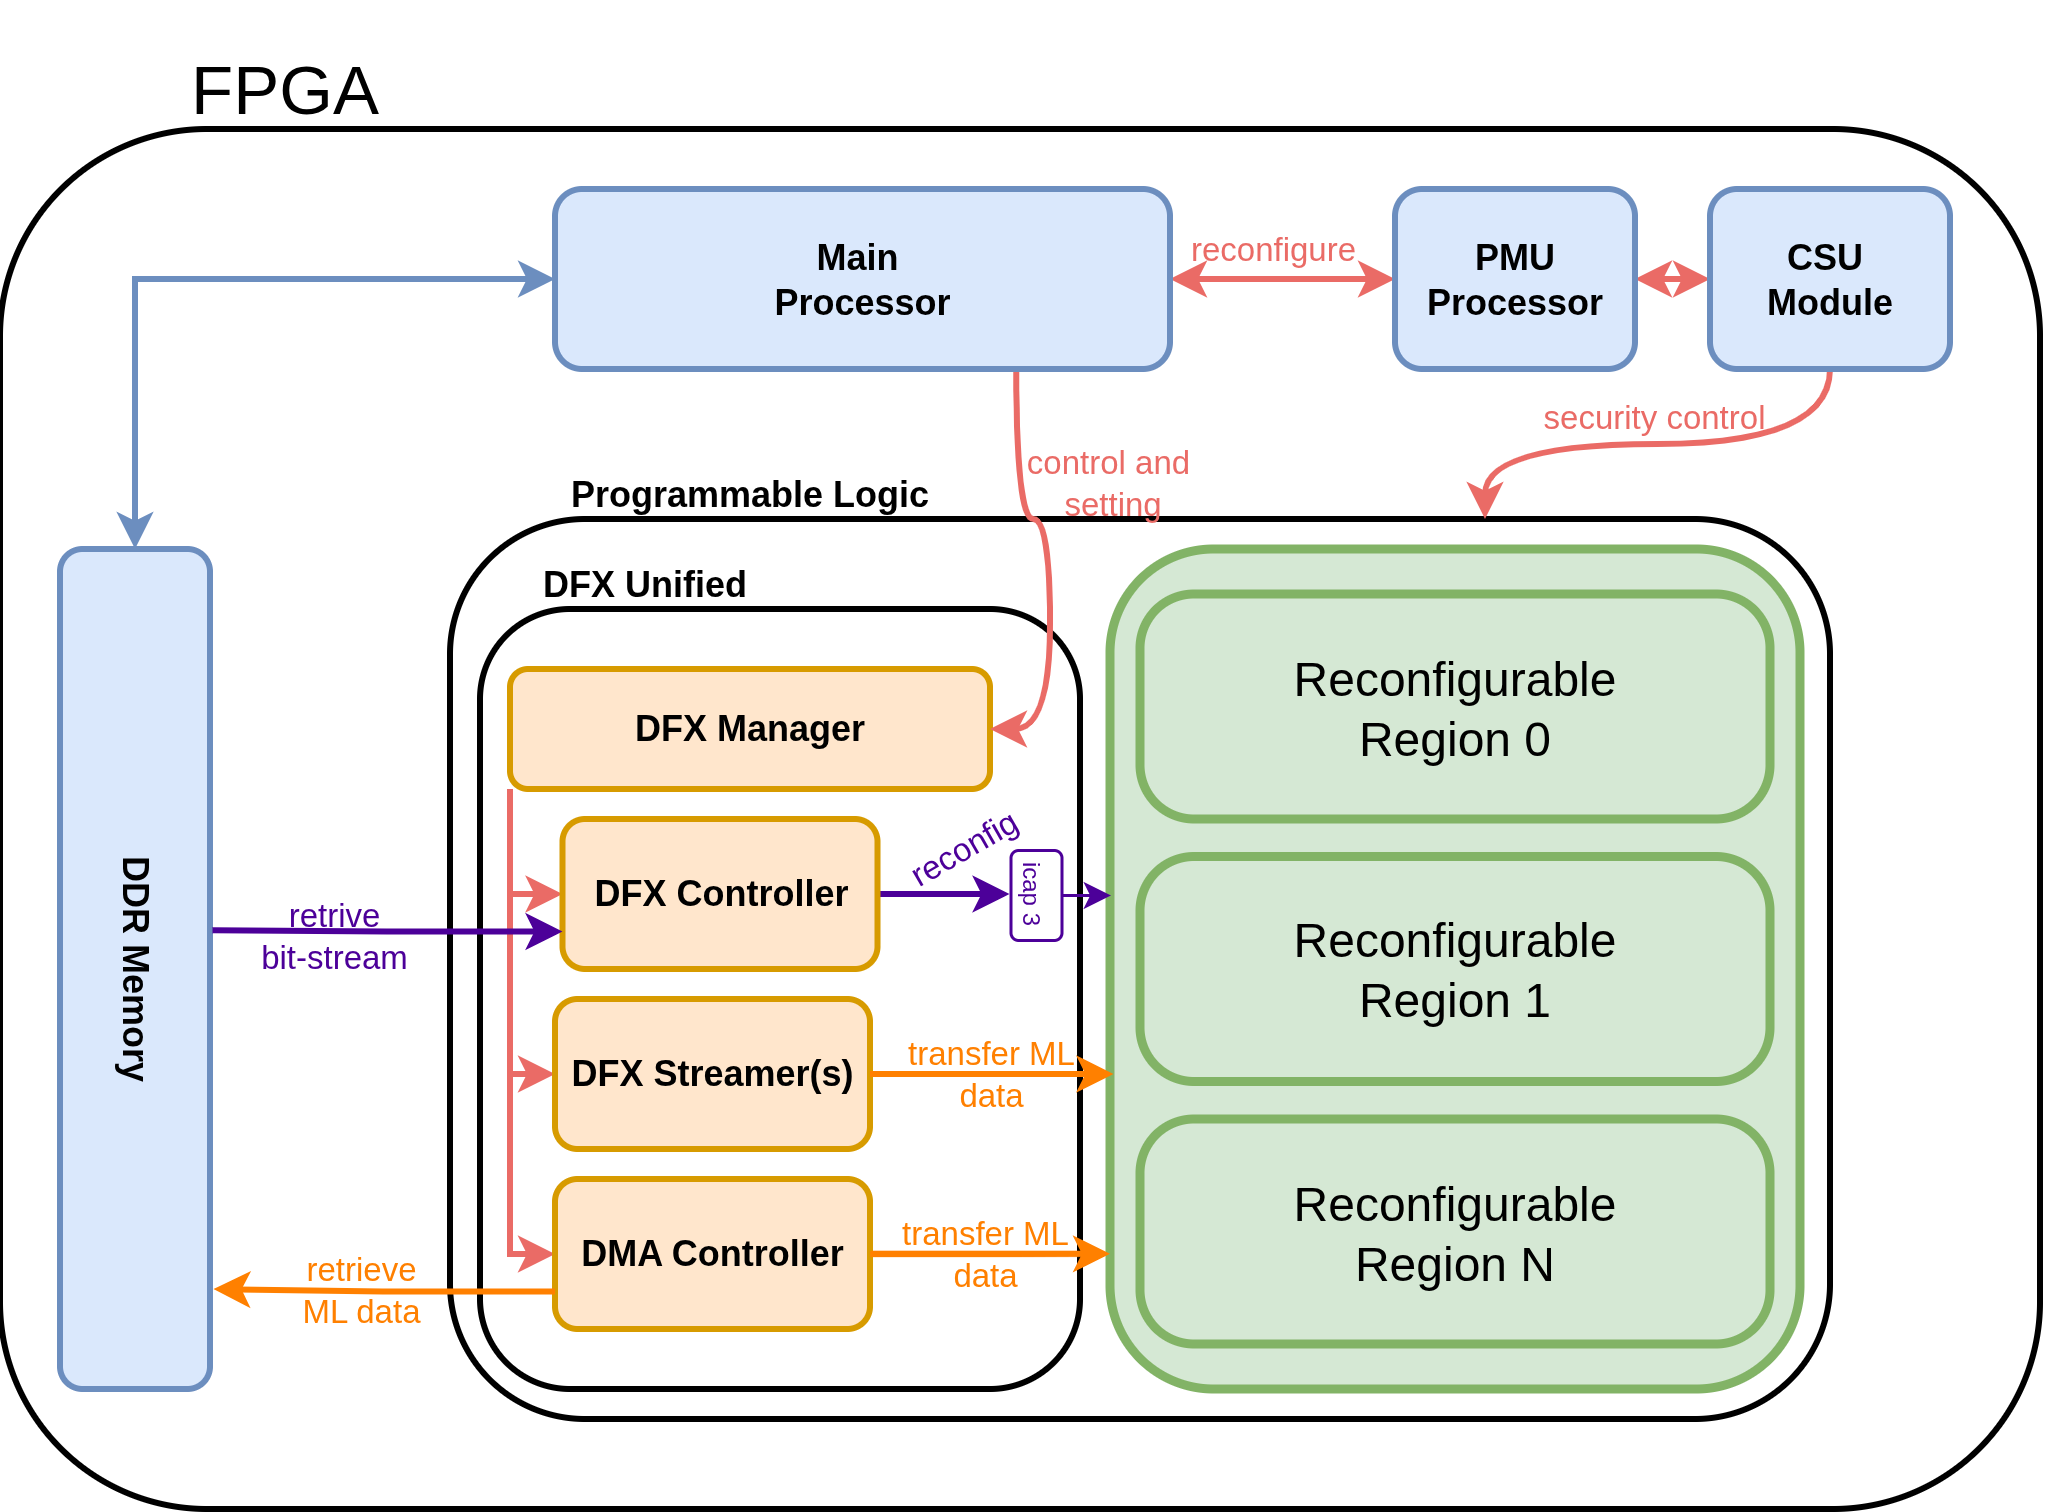
\includegraphics[width=0.8\textwidth]{images/overall_system.png}
\caption{\label{fig:overviewArch} DFX4ML-ARCH overall architecture}
\end{figure}

Fig.\ref{fig:overviewArch} illustrates the overall hardware architecture of DFX4ML-ARCH. The hardware architecture is composed of 4 major parts:

\begin{enumerate}
\item \textbf{Main Processor}. This project focuses on the Xilinx SoC with the PYNQ framework. The PYNQ framework allows users to manage memory allocation and initialization. Moreover, the processor is responsible for controlling Programmable Logic and communicating with the PMU processor.
\item \textbf{PMU and CSU}. The Platform Management Unit (PMU) and Control Security Unit (CSU) are the Xilinx SoC's management systems. The PMU is a dedicated processor used to manage the system's routine tasks and secure the system at the hardware level. In this project, we have to command the PMU to orchestrate the Programmable Logic permissions.
\item \textbf{Programmable Logic}. To support partial reconfiguration, the DFX4ML-ARCH is divided into 2 region:
  \begin{enumerate}
    \item \textbf{Static Region}. The region that is always active and contains the control logic and temporary memory storage. We propose four main components:
      \begin{enumerate}
        \item \textbf{DFX Manager}: it manages all PL components: (1) commands the DFX Controller, (2) controls the DFX Streamer, (3) controls the DMA Controller, (4) profiles the system, (5) interrupts the processor, and (6) receives commands and metadata from the processor.
        \item \textbf{DFX Controller}: This Xilinx IP receives commands from the DFX Manager. When it is triggered, the system loads the partial bitstream file from main memory (DDR RAM) and reprograms the partial region through the ICAP3 port.
        \item \textbf{DFX Streamer(s)}: it is the storage based on BRAM (on-chip memory) used to hold data temporarily while the partial region is reconfiguring.
        \item \textbf{DMA Controller}: this Xilinx IP is used to transfer data from DDR RAM directly to the partial region.
      \end{enumerate}
    \item \textbf{Reconfigurable Region (RP)}. This region is dedicated to machine learning workload. The input\/output only comes from the AXI-Stream.
  \end{enumerate}

\end{enumerate}



 
\subsection{DFX Manager}

DFX Manager is the IP used to orchestrate the entire Programmable Logic function. Fig.~\ref{fig:dfx_mng_arch} illustrates the overall components in the manager.

\begin{figure}[ht]
\centering
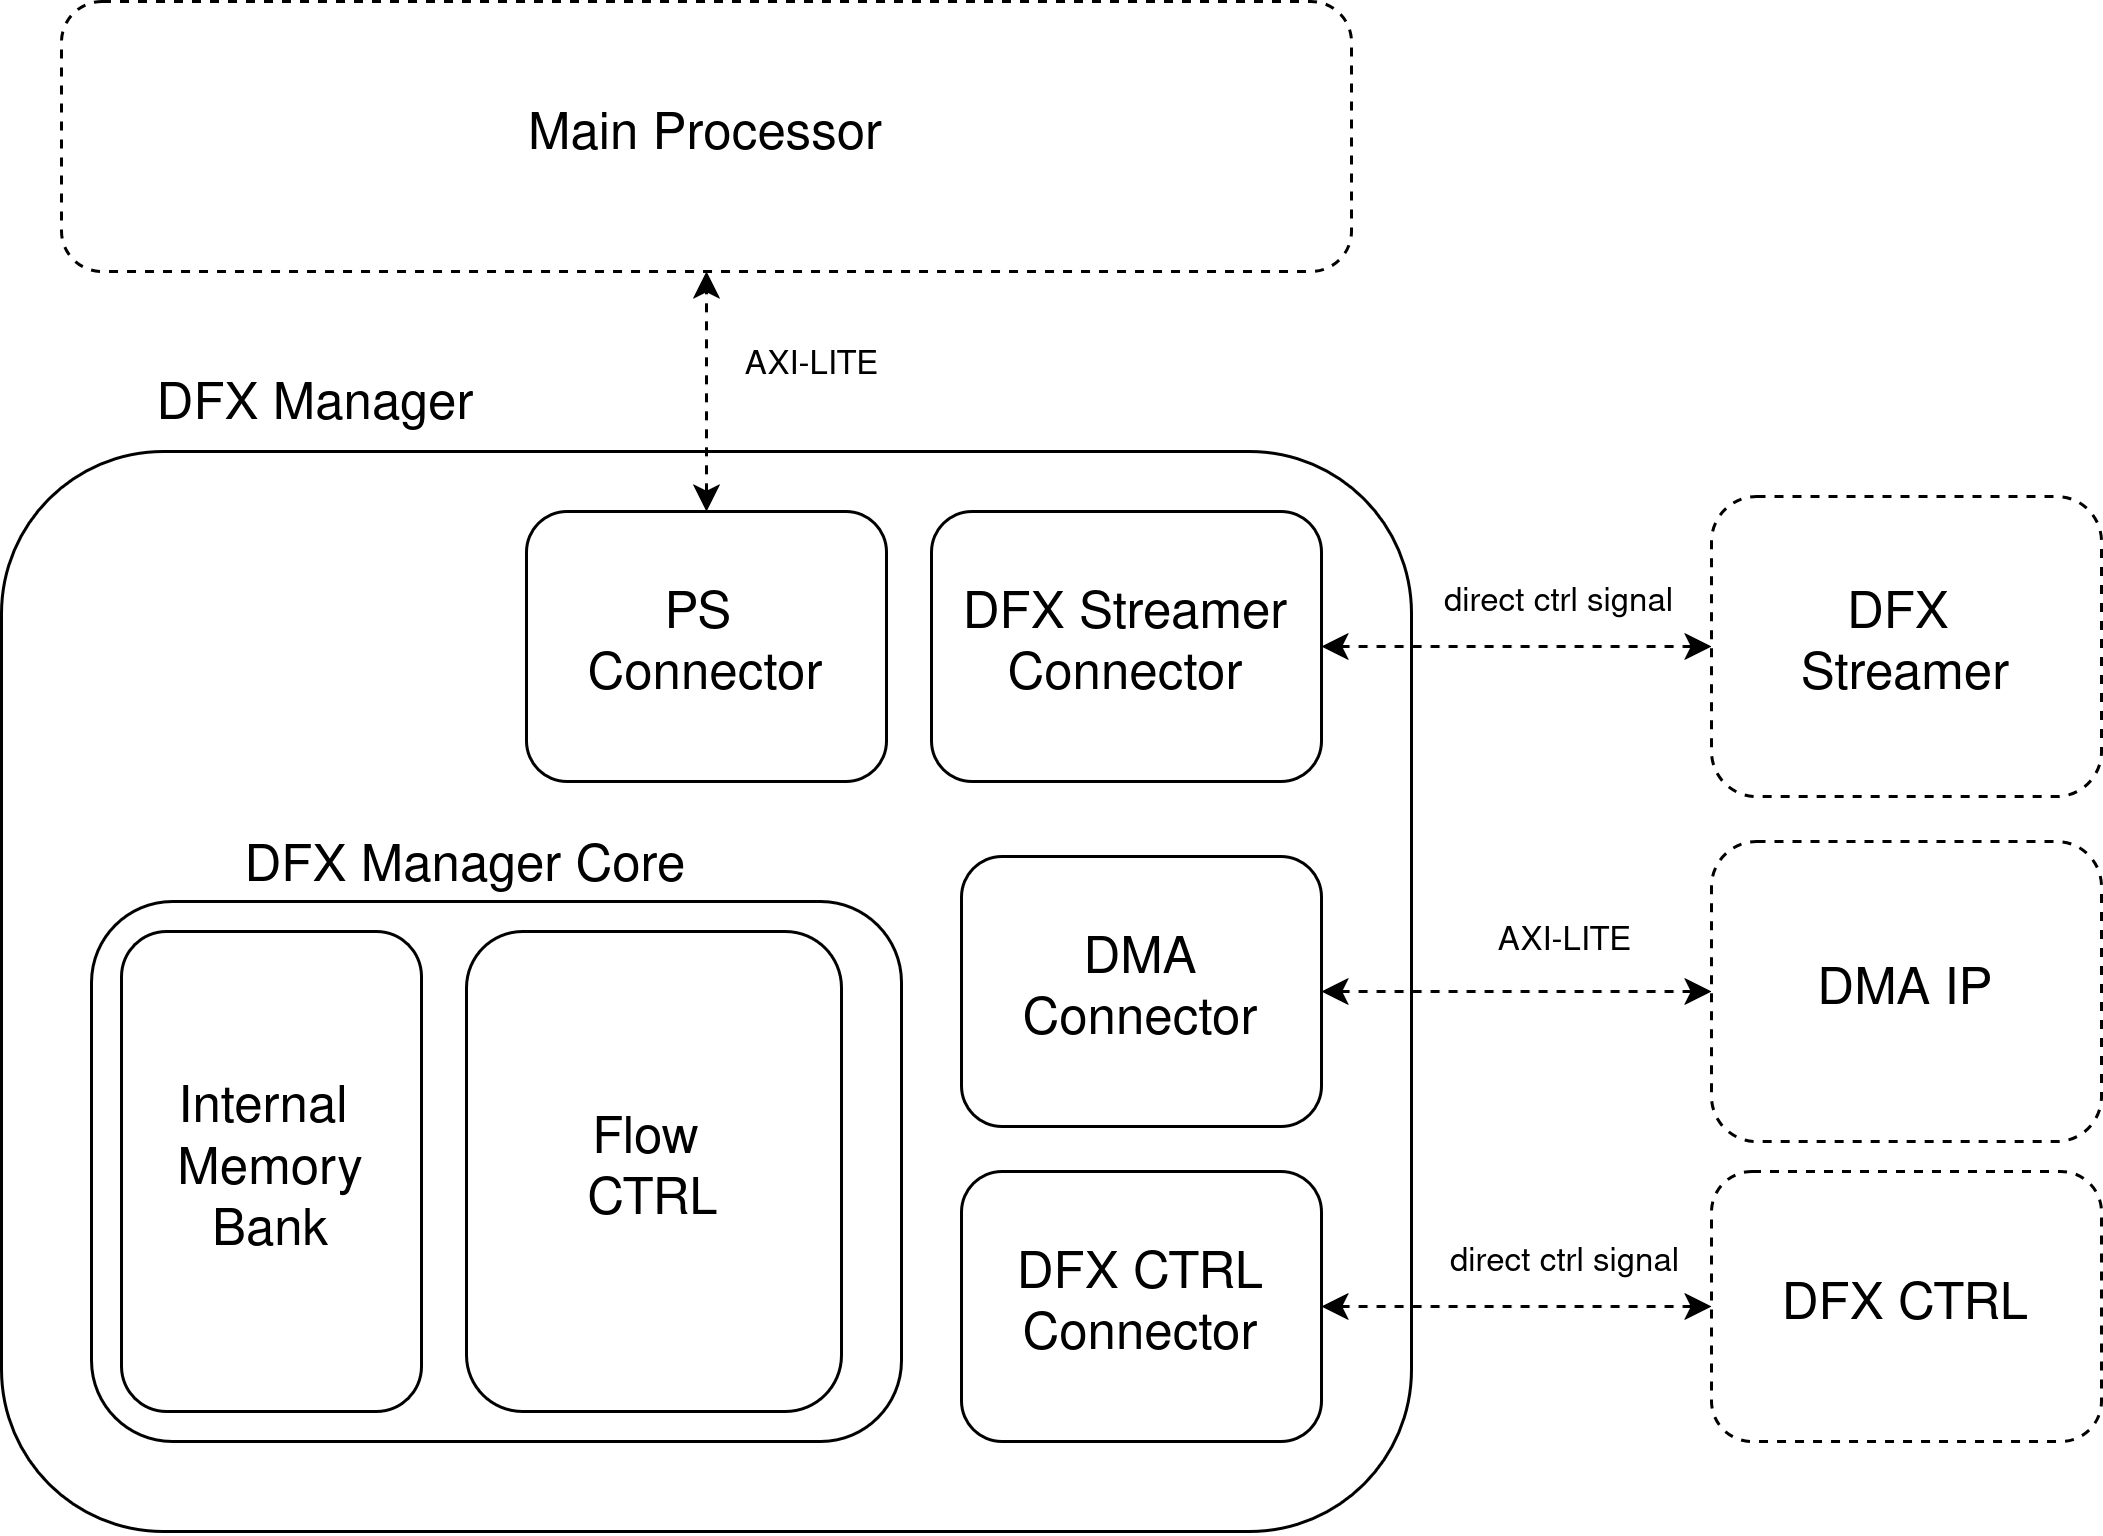
\includegraphics[width=0.8\textwidth]{images/dfx_mng_arch.png}
\caption{\label{fig:dfx_mng_arch} DFX Manager}
\end{figure}


The DFX Manager is composed of 5 major components:

\begin{enumerate}
  \item PS Connector: It communicates with the main processor (PS) through the AXI-LITE slave protocol. The code is at \textcolor{darkgreen}{\texttt{hw/ip\_src/dfx\_mng/s\_axi\_\{read,write\}.v}}
  \item DFX Streamer Connector: The connector directly passes signals from the DFX Manager Core through control signals to trigger load/store operations, and also receives the data-holding status from the streamers.
  \item DMA Connector: The DFX Manager Core requires multiple steps to set up the DMA controller properly; therefore, the DMA connector is responsible for managing the sequence of AXI-LITE packets sent to the DMA IP. The code is at\newline\textcolor{darkgreen}{\texttt{hw/ip\_src/dfx\_mng/m\_axi\_\{read,write\}.v}}
  \item DFX CTRL Connector: The connector directly passes signals from the DFX Manager Core through control signals to trigger the DFX CTRL IP to decouple and reconfigure the partial region. This connector also receives data back from the target IP to indicate that the reconfiguration is finished.
  \item DFX Manager Core: it contains the internal register memory used to control the flow of the system and provide data for the slave IPs. Moreover, Flow CTRL is responsible for orchestrating the slave IPs to work in the correct order.
\end{enumerate}

\subsubsection{DFX Manager's Reconfigurable Parameter}

The DFX Manager IP is parameterized at synthesis time via Verilog \texttt{parameter} declarations, allowing the designer to tailor its resource usage and functional scope to the target platform. Table~\ref{tab:dfx_mng_params} summarises all exposed parameters.
 

\rowcolors{2}{white}{headerbg}
\begin{longtable}{
    L{4.8cm}  % Parameter
    C{1.6cm}  % Default
    L{7.8cm}  % Description
}
\caption{DFX Manager Reconfigurable Parameters}
\label{tab:dfx_mng_params}\\
\toprule
\rowcolor{white}
\textbf{Parameter} & \textbf{Default} & \textbf{Description} \\
\midrule
\endfirsthead
\caption[]{DFX Manager Reconfigurable Parameters (continued)}\\
\toprule
\rowcolor{white}
\textbf{Parameter} & \textbf{Default} & \textbf{Description} \\
\midrule
\endhead
\bottomrule
\endfoot

% ── Global ──────────────────────────────────────────────────────────────────
\rowcolor{sectionbg} \multicolumn{3}{l}{\small\textbf{\textsc{Global}}} \\
\reg{GLOB\_ADDR\_WIDTH} & 32 & AXI address bus width. \\
\reg{GLOB\_DATA\_WIDTH} & 32 & AXI data bus width. \\
\reg{NUM\_REGION}       &  2 & Number of independently managed DFX reconfigurable regions. \\

% ── Bank 0 — Control & Status ───────────────────────────────────────────────
\rowcolor{sectionbg} \multicolumn{3}{l}{\small\textbf{\textsc{Bank 0 --- Control \& Status}}} \\
\reg{BANK0\_CONTROL\_WIDTH}  & 4  & The width of the control register \\
\reg{BANK0\_STATE\_BIT\_LEN} & 4  & state register width (recon\_state, exec\_state). \\
\reg{BANK0\_QUERY\_BIT\_LEN} & 32 & Query register bit width (bank0) \\ 

% ── Bank 1 — Slot & DMA Descriptor ─────────────────────────────────────────
\rowcolor{sectionbg} \multicolumn{3}{l}{\small\textbf{\textsc{Bank 1 --- Slot \& DMA Descriptor}}} \\
\reg{BANK1\_INDEX\_WIDTH}            &  3 & Session-index width; supports $2^{n}$ slots (default: 8). \\
\reg{BANK1\_DATA\_ADDR\_WIDTH}       & 32 & DMA start-address width per session. \\
\reg{BANK1\_DATA\_SIZE\_WIDTH}       & 26 & DMA transfer-size width (max $2^{26}$ bytes $\approx$ 64~MB). \\
\reg{BANK1\_RM\_SELECT\_WIDTH}       &  2 & RM-select width; encodes $N_{\mathrm{VS}} \times M_{\mathrm{RM/VS}}$ module variants. \\
\reg{BANK1\_PROFILE\_RECON\_WIDTH}   & 32 & Reconfiguration phase profiling counter width. \\
\reg{BANK1\_PROFILE\_EXEC\_WIDTH}    & 32 & Execution phase profiling counter width. \\
\reg{BANK1\_DATA\_POOL\_MASK\_WIDTH} & 8  & DFX Streamers (MGSs) selecting bit width\\

\end{longtable} 

\subsubsection{DFX Manager Core}

\paragraph{\textbf{Register Architecture (internal register bank)}}

\begin{figure}[ht]
\centering
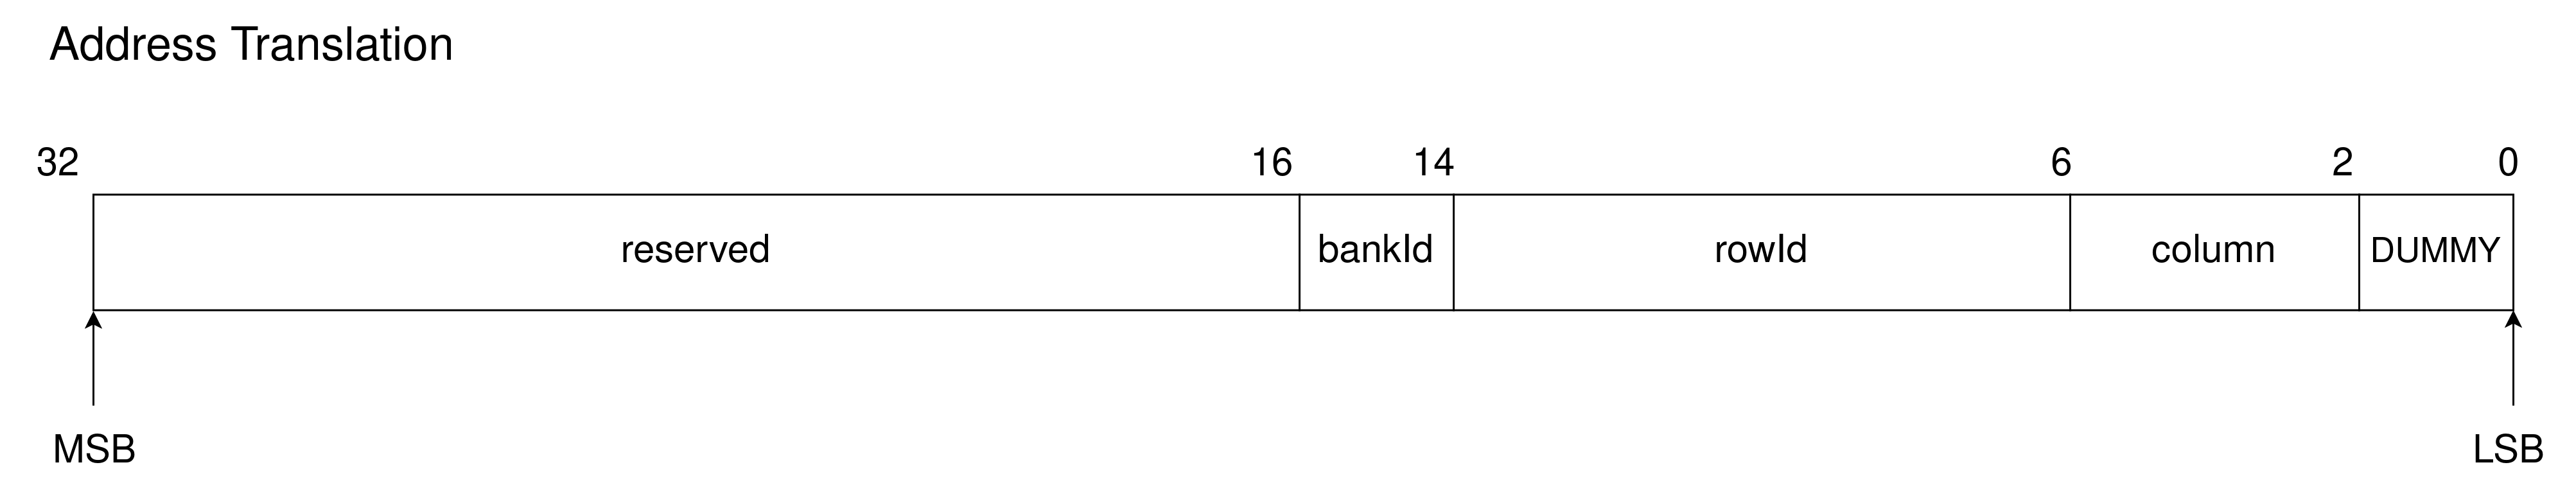
\includegraphics[width=1.0\textwidth]{images/dfx_mng_addr_tran.png}
\caption{\label{fig:dfx_mng_tran} DFX Manager Core's internal register address translation}
\end{figure}

We propose the register architecture that resides in the internal memory bank. Users can access these via memory-mapped I/O. The TCL build script sets the default address at $0xA000\_0000$ with a 64~KB address range.

With a 64~KB range, the address space is categorized into 3 main sections:

\begin{enumerate}
  \item \textbf{bankId} (bits 14--15): the system supports up to 4 banks. Each bank is a group of rows that belong to the same functional group.
  \item \textbf{rowId} (bits 13--6): each bank supports up to 256 rows. A row is a group of registers; however, different rows in the same bank do not have to follow the same schema.
  \item \textbf{column} (bits 5--2): each row supports up to 16 registers. Each register in the row does not have to be the same size. However, the register size must not exceed 4 bytes (32 bits).
\end{enumerate}

Fig.~\ref{fig:dfx_mng_reg} illustrates the DFX Manager's internal memory. The system is composed of two memory banks: Bank 0 is dedicated to IP control, the debugging system, overall running configuration, interrupt settings, and flow control memory; Bank 1 is composed of several rows sharing the same register pattern, used to store data and metadata for reconfigurable module initialization and slave static IP commands.
 
% =============================================================================
\paragraph{\textbf{Bank 0 — Global Control Registers}}

This bank is mainly used to control the flow control system and slave IP identifiers. It provides 13 registers accessible from the processor (PS) via the AXI-LITE protocol. Note that each Bank~0 register occupies a full row (64~B stride), since bits[13:6] select the row with no column multiplexing inside Bank~0. The code is at \textcolor{darkgreen}{\texttt{hw/ip\_src/dfx\_mng/dfx\_mng\_core.v}}

\vspace{1.0em}


\textit{Base offset: \addr{0x0000}}

\vspace{0.5em}

\rowcolors{2}{white}{headerbg}
\begin{longtable}{
    L{1.6cm}   % Address
    L{3.4cm}   % Register
    L{2.8cm}   % Width
    C{1.4cm}   % Access
    L{5.5cm}   % Description
}
\caption{Bank 0 — Global Control Registers}
\label{tab:bank0_registers}\\
\toprule
\rowcolor{white}
\textbf{Address} & \textbf{Register} & \textbf{Width} & \textbf{Access} & \textbf{Description} \\
\midrule
\endfirsthead
\caption[]{Bank 0 — Global Control Registers (continued)}\\
\toprule
\rowcolor{white}
\textbf{Address} & \textbf{Register} & \textbf{Width} & \textbf{Access} & \textbf{Description} \\
\midrule
\endhead
\bottomrule
\endfoot 

\addr{0x0000} & \reg{CTRL\_REG} & {\small\reg{BANK0\_CONTROL}\newline\reg{\_WIDTH}} & \badwo &
  Control register (write-only).\newline
  \textbf{0x0}~=~CLEAR (reset all state machines and counters)\newline
  \textbf{0x1}~=~SHUTDOWN (halt gracefully)\newline
  \textbf{0x2}~=~START (begin processing) \\

\addr{0x0040} & \reg{MAIN\_STATE} & {\small\reg{BANK0\_STATE}\newline\reg{\_BIT\_LEN}} & \badro &
  Main flow state machine output:\newline
  \textbf{0x0}~=~SHUTDOWN\newline
  \textbf{0x1}~=~PROCESS\newline
  \textbf{0x2}~=~PRE\_SHUTDOWN \\

\addr{0x0080} & \reg{RECON\_STATE} & {\small\reg{BANK0\_STATE}\newline\reg{\_BIT\_LEN}} & \badro &
  Reconfiguration sub-state machine (runs in parallel with \reg{EXEC\_STATE}):\newline
  \textbf{0x0}~=~SHUTDOWN\newline
  \textbf{0x1}~=~REPROG\newline
  \textbf{0x2}~=~W4SLAVERESET\newline
  \textbf{0x3}~=~W4SLAVEOP\newline
  \textbf{0x4}~=~FIN\_SYNC \\

\addr{0x00C0} & \reg{EXEC\_STATE} & {\small\reg{BANK0\_STATE}\newline\reg{\_BIT\_LEN}} & \badro &
  Execution sub-state machine (runs in parallel with \reg{RECON\_STATE}):\newline
  \textbf{0x0}~=~SHUTDOWN\newline
  \textbf{0x1}~=~INITIALIZE\_PR\_CTRL\newline
  \textbf{0x2}~=~CLEAR\_MGS\newline
  \textbf{0x3}~=~INITIALIZE\_MGS\newline
  \textbf{0x4}~=~INITIALIZE\_DMA\newline
  \textbf{0x5}~=~SET\_DMA\_LOAD\newline
  \textbf{0x6}~=~SET\_DMA\_STORE\newline
  \textbf{0x7}~=~TRIGGERING\newline
  \textbf{0x8}~=~WAIT4FIN\newline
  \textbf{0x9}~=~FIN\_SYNC \\

\addr{0x0100} & \reg{LAST\_SESSION} & {\small\reg{BANK1\_INDEX}\newline\reg{\_WIDTH}} & \badrw &
  Index of the last session in the execution round. The main machine stops cycling when the current session index equals this value and the query budget is exhausted. \\

\addr{0x0140} & \reg{CUR\_QUERY} & {\small\reg{BANK0\_QUERY}\newline\reg{\_BIT\_LEN}} & \badro &
  Current query counter. Incremented by \reg{AMT\_QUERY\_PER\_ITER} after each full session round. Cleared on CLEAR or START. \\

\addr{0x0180} & \reg{AMT\_QUERY} & {\small\reg{BANK0\_QUERY}\newline\reg{\_BIT\_LEN}} & \badrw &
  Total query budget. The system shuts down automatically when \reg{CUR\_QUERY} reaches this value. \\

\addr{0x01C0} & \reg{AMT\_QUERY} \newline \reg{\_PER\_ITER} & {\small\reg{BANK0\_QUERY}\newline\reg{\_BIT\_LEN}} & \badrw &
  Number of queries processed per iteration (per full session round). Added to \reg{CUR\_QUERY} on each round completion. \\

\addr{0x0200} & \reg{DMA\_IP\_ADDR} & {\small\reg{GLOB\_ADDR\_WIDTH}} & \badrw &
  Base address of the DMA IP in the memory-mapped peripheral space. Used by the DMA Connector to issue AXI-LITE transactions. \\

\addr{0x0240} & \reg{PR\_IP\_ADDR} & {\small\reg{GLOB\_ADDR\_WIDTH}} & \badrw &
  Base address of the PR-controlled IP (e.g., the ML accelerator) in the peripheral space. Used by the PR CTRL Connector to initialize the IP via \texttt{batch\_size} and \texttt{ap\_start}. \\

\addr{0x0280} & \reg{INTR\_ENA} & 1 bit & \badrw &
  Interrupt enable. Set to \textbf{1} to assert the interrupt line when all queries finish. \\

\addr{0x02C0} & \reg{INTR\_STATUS} & 1 bit & \badro &
  Interrupt status. Set to \textbf{1} when \reg{CUR\_QUERY}~$=$~\reg{AMT\_QUERY}. Cleared on CLEAR or START. \\

\addr{0x0300} & \reg{MPERF} & {\small\reg{BANK0\_QUERY}\newline\reg{\_BIT\_LEN}} & \badrw &
  Global performance counter. Increments every clock cycle while \reg{RECON\_STATE} or \reg{EXEC\_STATE} is not in SHUTDOWN, measuring total engine-busy cycles across a run. Writable from the PS while the system is in SHUTDOWN (like the other R/W Bank~0 registers); cleared on hardware reset. \\

\end{longtable}

\vspace{1em}

% =============================================================================
\paragraph{\textbf{Bank 1 — Reconfigurable Module Slot Registers}}

This bank stores per-session data and metadata. Each row (session slot) follows a uniform 12-register pattern and contains DMA transfer parameters, profiling counters, RM selection fields, I/O stream masks, and a linked-list \reg{NEXT\_SESSION} pointer. The session execution order is defined by the \reg{NEXT\_SESSION} chain rather than contiguous row indices. The code is at \textcolor{darkgreen}{\texttt{hw/ip\_src/dfx\_mng/dfx\_mng\_core.v}}


\textit{Base offset: \addr{0x4000 + 0x40*session\_i}}

\vspace{0.5em}

\rowcolors{2}{white}{headerbg}
\begin{longtable}{
    L{1.6cm}   % Slot Offset
    L{3.4cm}   % Register
    L{2.8cm}   % Width
    C{1.4cm}   % Access
    L{5.5cm}   % Description
}
\toprule
\rowcolor{white}
\textbf{Slot Offset} & \textbf{Register} & \textbf{Width} & \textbf{Access} & \textbf{Description} \\
\midrule
\endfirsthead
\toprule
\rowcolor{white}
\textbf{Slot Offset} & \textbf{Register} & \textbf{Width} & \textbf{Access} & \textbf{Description} \\
\midrule
\endhead
\bottomrule
\endfoot

% ── DMA Source ────────────────────────────────────────────────────────────────
\subrow{DMA Transfer — Source}

\addr{+0x00} & \reg{DMA\_SRC\_ADDR} & {\small\reg{BANK1\_DATA}\newline\reg{\_ADDR\_WIDTH}} & \badrw &
  Source memory address. Address in system memory from which the DMA engine reads data for this session. \\

\addr{+0x04} & \reg{DMA\_SRC\_SIZE} & {\small\reg{BANK1\_DATA}\newline\reg{\_SIZE\_WIDTH}} & \badrw &
  Source transfer size in bytes for this session. \\

% ── DMA Destination ───────────────────────────────────────────────────────────
\subrow{DMA Transfer — Destination}

\addr{+0x08} & \reg{DMA\_DES\_ADDR} & {\small\reg{BANK1\_DATA}\newline\reg{\_ADDR\_WIDTH}} & \badrw &
  Destination memory address. Address in system memory where the DMA engine writes output data for this session. \\

\addr{+0x0C} & \reg{DMA\_DES\_SIZE} & {\small\reg{BANK1\_DATA}\newline\reg{\_SIZE\_WIDTH}} & \badrw &
  Destination transfer size in bytes for this session. \\

% ── Profiling ─────────────────────────────────────────────────────────────────
\subrow{Profiling Counters}

\addr{+0x10} & \reg{PROF\_RECON} & {\small\reg{BANK1\_PROFILE}\newline\reg{\_RECON\_WIDTH}} & \badrw &
  Reconfiguration profiler counter. Auto-incremented every cycle while \reg{RECON\_STATE} is in REPROG, W4SLAVERESET, or W4SLAVEOP. PS may write to reset or preset the counter. \\

\addr{+0x14} & \reg{PROF\_EXEC} & {\small\reg{BANK1\_PROFILE}\newline\reg{\_EXEC\_WIDTH}} & \badrw &
  Execution profiler counter. Auto-incremented every cycle while \reg{EXEC\_STATE} is in any active (non-SHUTDOWN / non-FIN\_SYNC) state. PS may write to reset or preset the counter. \\

% ── RM Selection ──────────────────────────────────────────────────────────────
\subrow{RM Selection}

\addr{+0x18} & \reg{VS\_RM\_RECON} \newline \reg{\_SELECT} & {\small\reg{BANK1\_RM}\newline\reg{\_SELECT\_WIDTH}} & \badrw &
  Selects which reconfigurable module to program during RECON. Forwarded to the DFX CTRL IP as the \texttt{dfx\_rm\_program} signal. \\

\addr{+0x1C} & \reg{VS\_RM\_EXEC} \newline \reg{\_SELECT} & {\small\reg{BANK1\_RM}\newline\reg{\_SELECT\_WIDTH}} & \badrw &
  Selects which RM the execution pipeline targets. Allows a different RM to be reconfigured while another executes. \\

% ── Stream Masks ──────────────────────────────────────────────────────────────
\subrow{Stream Masks}

\addr{+0x20} & \reg{LOAD\_MASK} & {\small\reg{BANK1\_DATA\_POOL}\newline\reg{\_MASK\_WIDTH}} & \badrw &
  Bit mask of input streamers that must be loaded before this session may execute. Bit~0 (LSB) is reserved for DMA; bits~1--7 correspond to DFX Streamer channels~1--7. \\

\addr{+0x24} & \reg{STORE\_MASK} & {\small\reg{BANK1\_DATA\_POOL}\newline\reg{\_MASK\_WIDTH}} & \badrw &
  Bit mask of output streamers that must store data after execution. Bit~0 (LSB) is reserved for DMA; bits~1--7 correspond to DFX Streamer channels~1--7. \\

\addr{+0x28} & \reg{COMPLETE\_MASK} & {\small\reg{BANK1\_DATA\_POOL}\newline\reg{\_MASK\_WIDTH}} & \badrw &
  Tracks which store operations have completed (same bit layout as \reg{STORE\_MASK}). Bits are ORed in automatically as streamers finish (\texttt{dfx\_stream\_fin}). The session is complete when \reg{COMPLETE\_MASK}~$=$~\reg{STORE\_MASK}. \\

% ── Linked List ───────────────────────────────────────────────────────────────
\subrow{Session Linked List}

\addr{+0x2C} & \reg{NEXT\_SESSION} & {\small\reg{BANK1\_INDEX}\newline\reg{\_WIDTH}} & \badrw &
  Index of the next session slot to execute after this one. Forms a singly-linked list of sessions; a round ends when the current slot index equals \reg{LAST\_SESSION} in Bank~0. \\

\end{longtable}

\vspace{1em}


\vspace{0.5em}

\paragraph{\textbf{Access Permission Legend}} 

\begin{tabular}{lll}
  \badrw & Read / Write & Register can be both read and written by the host. \\[4pt]
  \badro & Read Only    & Register is read-only; writes are ignored. \\[4pt]
  \badwo & Write Only   & Register is write-only; reads return undefined values. \\
\end{tabular}

\vspace{1.5em}

\begin{figure}[ht]
\centering
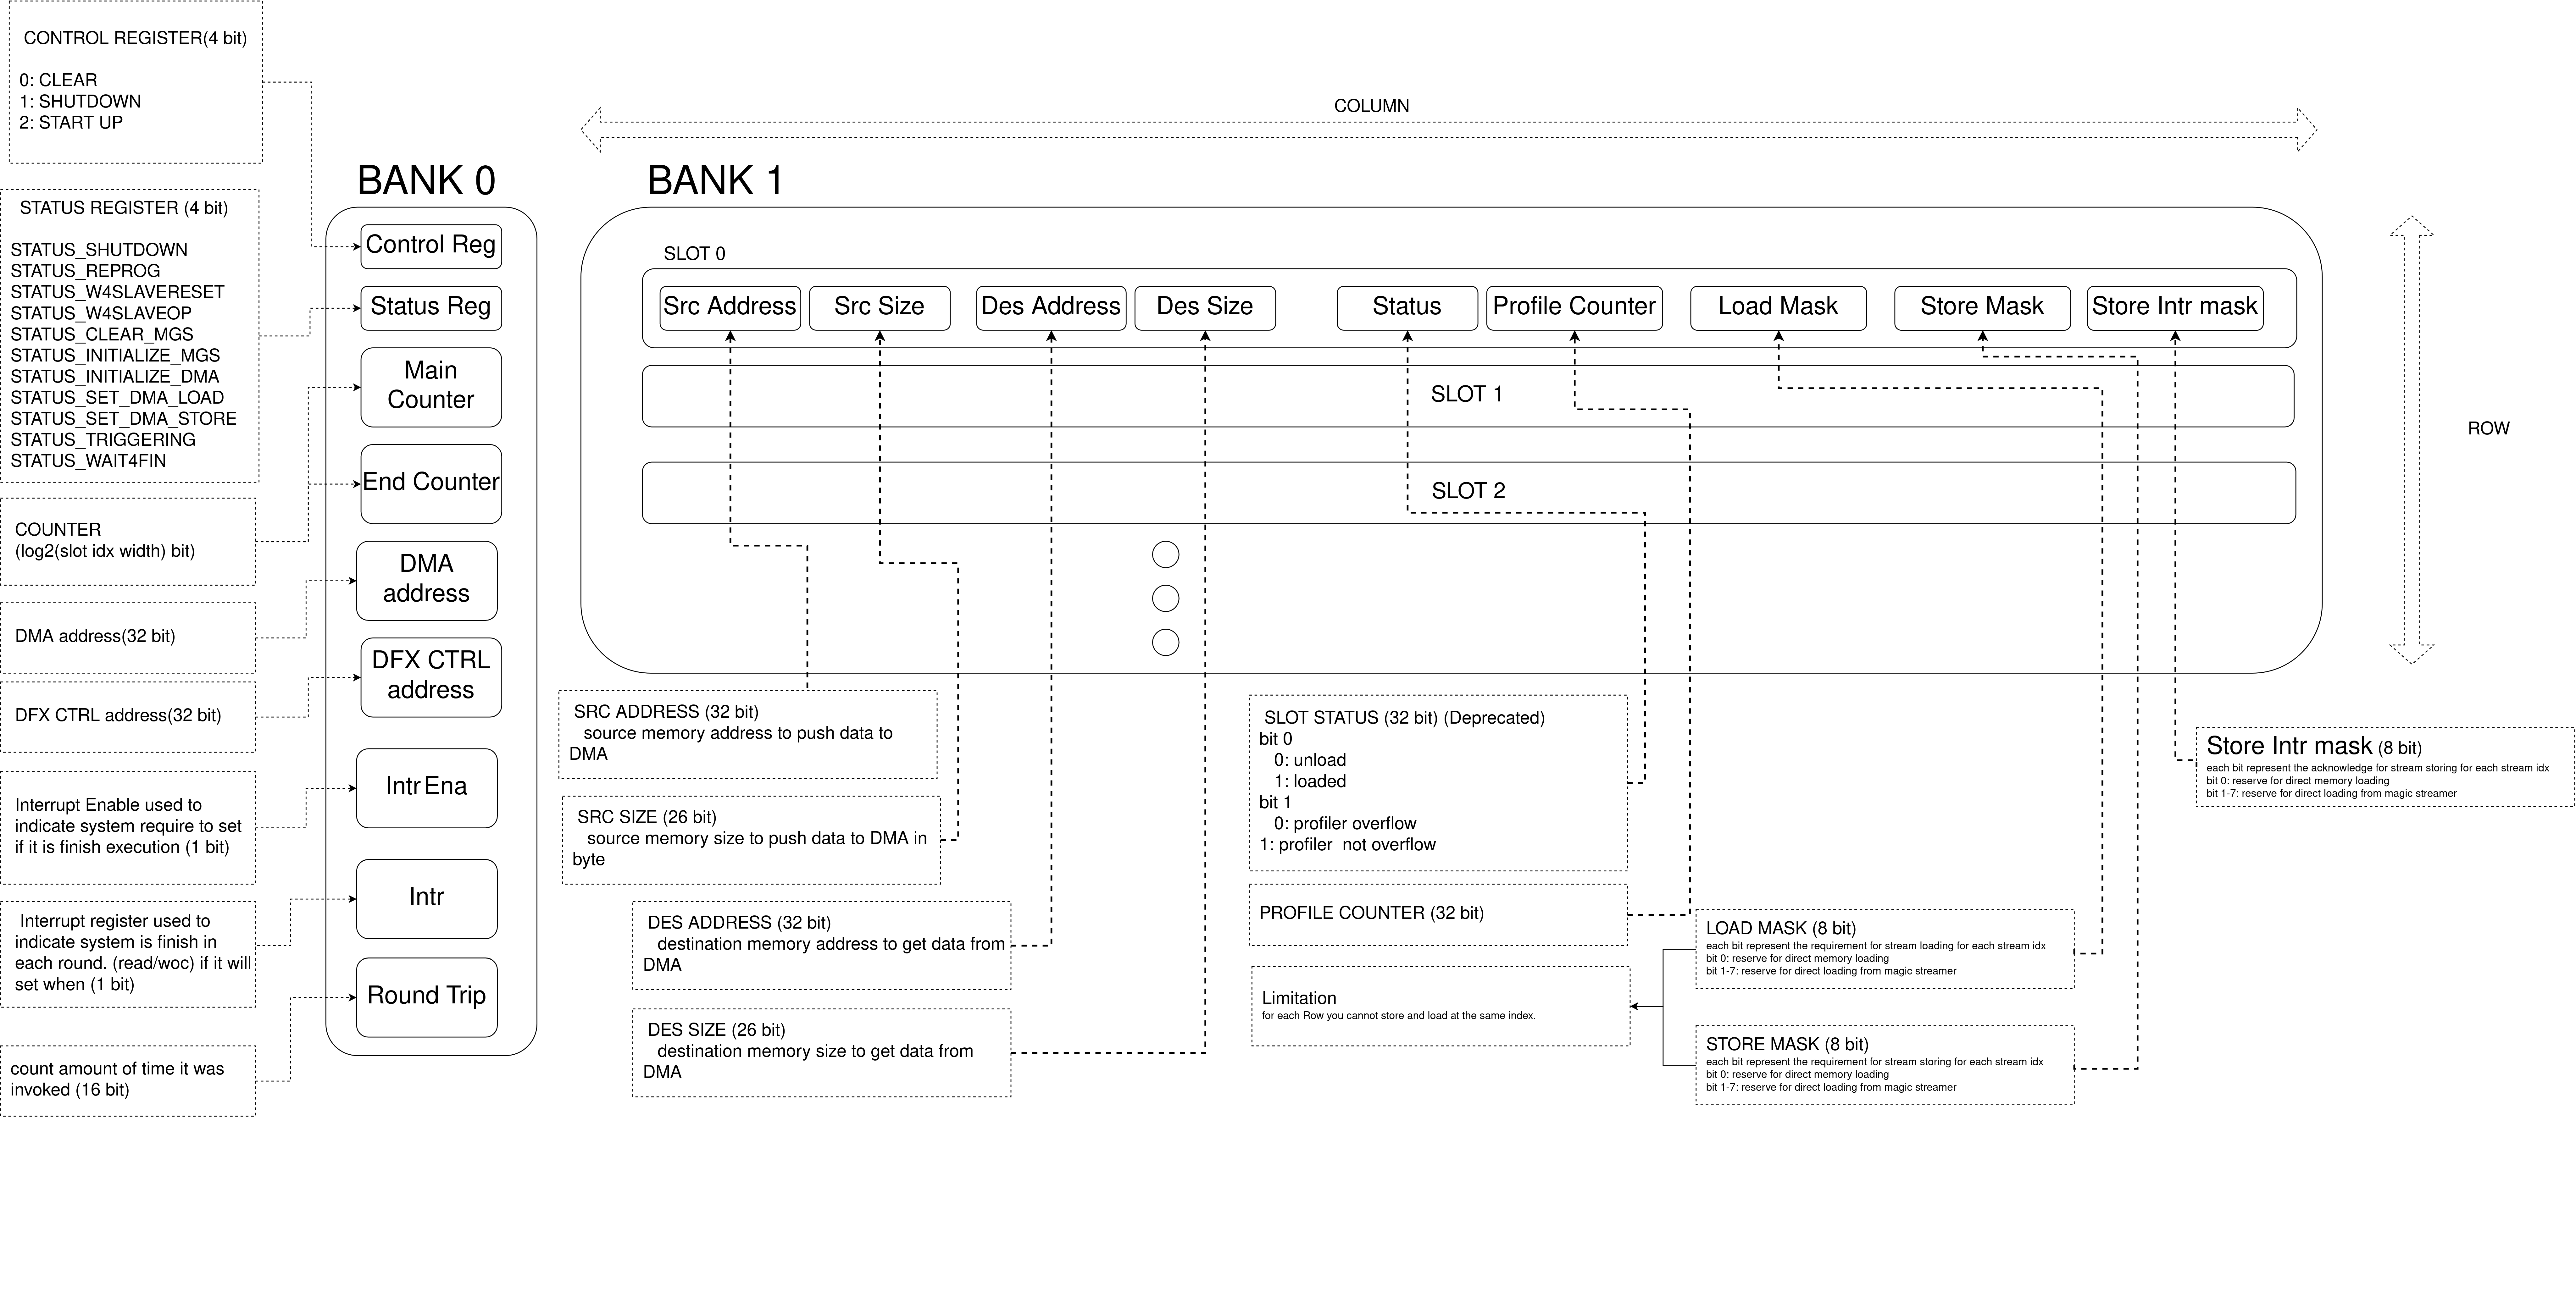
\includegraphics[width=0.8\textwidth]{images/dfx_mng_reg.png}
\caption{\label{fig:dfx_mng_reg} DFX Manager Core's internal register overview}
\end{figure}


\paragraph{\textbf{Flow Control (state machine)}}

Flow Control orchestrates the slave IP steps --- DFX Controller, DMA IP, and DFX Streamer (formerly Magic Streamer) --- to execute initialization and operation commands sequentially at the cycle-accurate level. The code is at \textcolor{darkgreen}{\texttt{hw/ip\_src/dfx\_mng/dfx\_mng\_core.v}}.
 
The DFX Manager Core runs three concurrent, loosely-coupled state machines whose outputs are readable from Bank~0 via \reg{MAIN\_STATE}, \reg{RECON\_STATE}, and \reg{EXEC\_STATE}. Fig.~\ref{fig:dfx_mng_state} illustrates the high-level state diagram.

\rowcolors{2}{white}{headerbg}
\begin{longtable}{
    L{4.0cm}   % State 
    L{9.8cm}   % Description
}
\caption{DFX Manager Flow Control --- State Machine Summary}
\label{tab:dfx_mng_states}\\
\toprule
\rowcolor{white}
\textbf{State} & \textbf{Description} \\
\midrule
\endfirsthead
\caption[]{DFX Manager Flow Control --- State Machine Summary (continued)}\\
\toprule
\rowcolor{white}
\textbf{State} & \textbf{Description} \\
\midrule
\endhead
\bottomrule 
\endfoot

% ── 1. Main state machine ─────────────────────────────────────────────────────
\rowcolor{sectionbg} \multicolumn{2}{l}{\small\textbf{\textsc{1.~Main State Machine (\reg{MAIN\_STATE})}}} \\
\reg{SHUTDOWN}      & Idle; Bank~0/1 registers are PS-writable. Waits for \reg{CTRL\_REG}~$=$~\texttt{CTRL\_START}. \\
\reg{PROCESS}       & Launches RECON and EXEC in parallel; holds until both reach \reg{FIN\_SYNC} simultaneously. \\
\reg{PRE\_SHUTDOWN} & Single-cycle housekeeping --- advances the session pointer (\reg{NEXT\_SESSION}), increments DMA addresses, then either loops back to \reg{PROCESS} or returns to \reg{SHUTDOWN}. Asserts \reg{INTR\_STATUS} if \reg{INTR\_ENA} is set and all queries are complete. \\

% ── 2. Reconfiguration sub-machine ───────────────────────────────────────────
\rowcolor{sectionbg} \multicolumn{2}{l}{\small\textbf{\textsc{2.~Reconfiguration Sub-machine (\reg{RECON\_STATE})}}} \\
\reg{REPROG}        & Reads \reg{VS\_RM\_RECON\_SELECT} from Bank~1.\newline
                      $\bullet$~If~$0$: skip to \reg{FIN\_SYNC} (bypasses W4SLAVERESET and W4SLAVEOP).\newline
                      $\bullet$~Otherwise: drives \texttt{dfx\_rm\_program} $\to$ \reg{W4SLAVERESET}. \\
\reg{W4SLAVERESET}  & Waits for \texttt{dfx\_rm\_nreset} to deassert. \\
\reg{W4SLAVEOP}     & Waits for \texttt{dfx\_rm\_nreset} to reassert (reconfiguration complete). \\
\reg{FIN\_SYNC}     & Holds until EXEC also reaches \reg{FIN\_SYNC}; both return to \reg{SHUTDOWN} together. \\

% ── 3. Execution sub-machine ─────────────────────────────────────────────────
\rowcolor{sectionbg} \multicolumn{2}{l}{\small\textbf{\textsc{3.~Execution Sub-machine (\reg{EXEC\_STATE})}}} \\
\reg{PR\_CTRL\_REQ} \newline \reg{\_SKIP\_CHECK} &
                      Entry state; reads \reg{VS\_RM\_EXEC\_SELECT} from Bank~1.\newline
                      $\bullet$~If~$0$: skip to \reg{CLEAR\_MGS}.\newline
                      $\bullet$~Otherwise: arm PR CTRL sequencer $\to$ \reg{INITIALIZE\_PR\_CTRL}. \\
\reg{INITIALIZE} \newline \reg{\_PR\_CTRL}    & Sends \texttt{batch\_size} and \texttt{ap\_start} to the PR-controlled IP (\reg{PR\_IP\_ADDR}); advances on \texttt{AP\_START} completion. \\
\reg{CLEAR\_MGS}    & One-cycle reset of DFX Streamer channels in \reg{LOAD\_MASK}. \\
\reg{INITIALIZE\_MGS} & One-cycle init of DFX Streamer channels in \reg{STORE\_MASK}. \\
\reg{INITIALIZE\_DMA} & Resets the DMA interrupt flag. \\
\reg{SET\_DMA\_LOAD}  & Programs DMA source address and size (\reg{DMA\_SRC\_ADDR}, \reg{DMA\_SRC\_SIZE}); skipped if \reg{LOAD\_MASK}[0]~$= 0$. \\
\reg{SET\_DMA\_STORE} & Programs DMA destination address and size (\reg{DMA\_DES\_ADDR}, \reg{DMA\_DES\_SIZE}); skipped if \reg{STORE\_MASK}[0]~$= 0$. \\
\reg{TRIGGERING}    & One-cycle state delayed (reserved for future used). \\
\reg{WAIT4FIN}      & Waits until \reg{COMPLETE\_MASK}~$=$~\reg{STORE\_MASK}. \\
\reg{FIN\_SYNC}     & Holds until RECON also reaches \reg{FIN\_SYNC}; both return to \reg{SHUTDOWN} together. \\

\end{longtable}

\begin{figure}[H] 
\centering
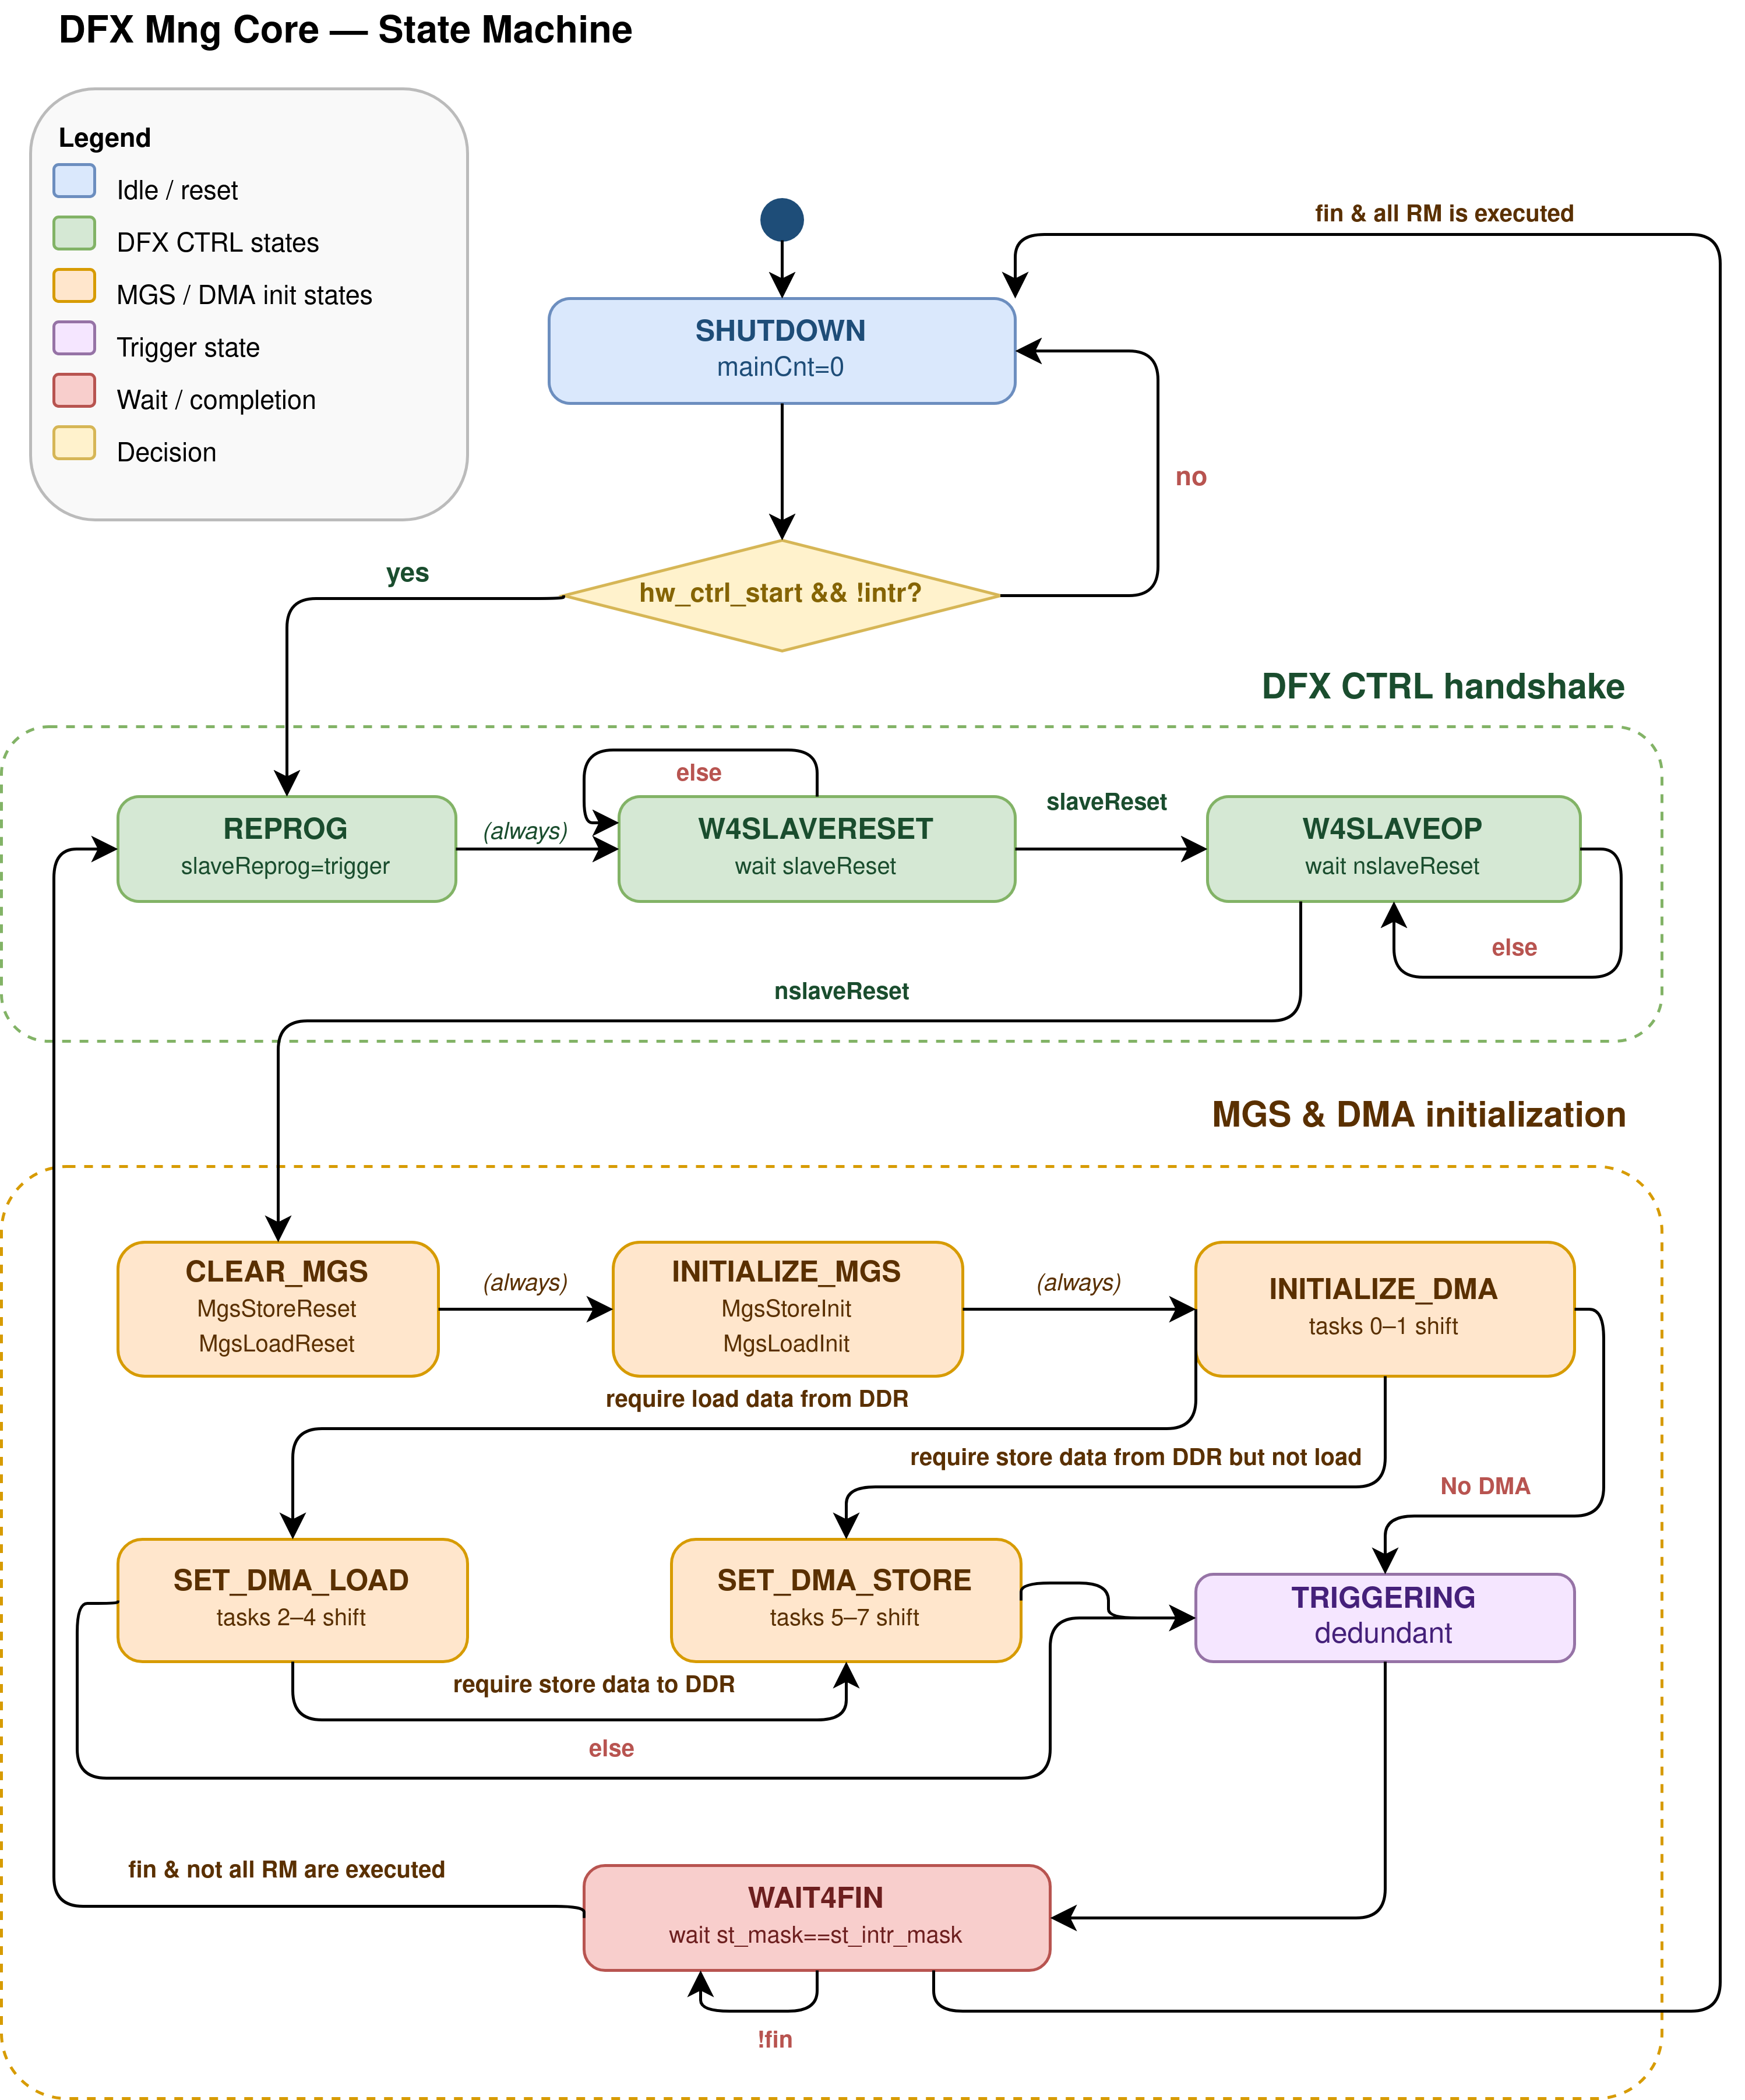
\includegraphics[width=0.95\textwidth]{images/dfx_mng_state_diagram.png}
\caption{\label{fig:dfx_mng_state} DFX Manager flow control (state diagram)}
\end{figure}



\subsection{DFX Streamer(s)}

DFX Streamer(s) is the temporary storage residing in the Programmable Logic static region and was designed to utilize BRAM resources for storage and a small number of flip-flops to hold its transfer metadata. The code is at \textcolor{darkgreen}{\texttt{hw/ip\_src/dfx\_streamer/dfx\_streamer.v}}

\begin{figure}[H]
\centering
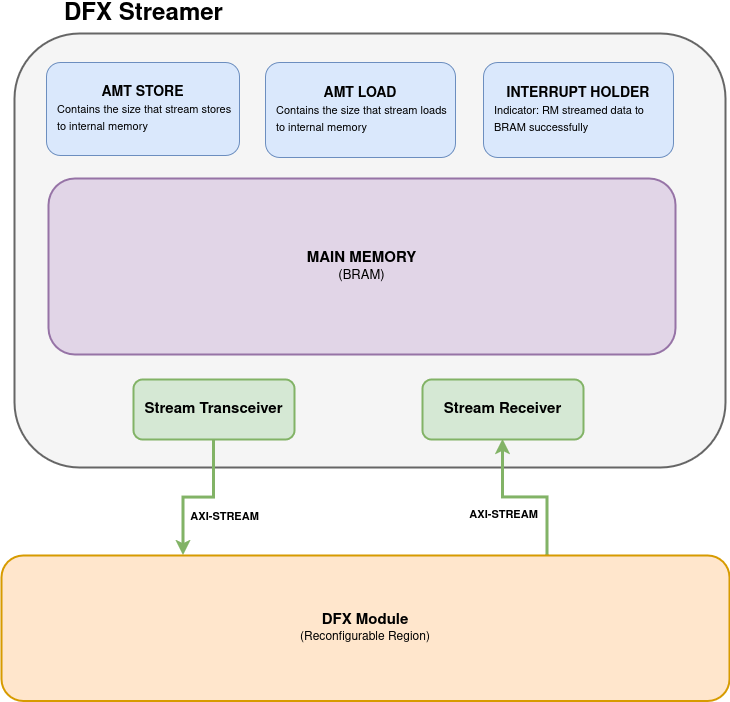
\includegraphics[width=0.65\textwidth]{images/dfx_streamer.png}
\caption{\label{fig:dfx_streamer} DFX Streamer Architecture}
\end{figure}

Fig.~\ref{fig:dfx_streamer} illustrates the overall architecture of the DFX Streamer. The \textbf{meta-data blocks} (blue boxes) reside in the static region, using flip-flops to track the amount of load/store operations and RM status (INTERRUPT HOLDER). Meanwhile, the \textbf{MAIN MEMORY} (purple block) also resides in the static region, but uses BRAM to store the temporary data.

The DFX Streamer's main memory packs 4096 entries per bank to maximise resource utilisation for each URAM. If entries are not packed, Vivado cannot decide to merge two memory banks into a single URAM/BRAM, even when they are not accessed simultaneously.

To address the latency problem, we pipeline the URAM/BRAM data transfer (both load and store). On the store side, we add an additional register equal to the wrap size to buffer data coming from the dynamic region. On the load side, we add an additional register equal to wrap size × number of memory banks; the pipeline supports back-pressure in case the ML model is not ready to receive data from the memory bank.

In contrast, the Stream Transceiver and Stream Receiver connection ports are open to the partial region via the \textbf{AXI-STREAM} interface. In the current version, the AXI-STREAM \textbf{tkeep} and \textbf{tlast} signals are \textbf{mandatory}. If they are not set up, the system will get stuck.

To support the parallel execution between (\textbf{Latency Hiding Technique}), the stream transceiver and stream receiver have their own dedicated DFX Decoupler (red box); therefore, it enables the DFX Streamer operating while there are reconfiguring modules.

\subsection{DFX\_CTRL}

DFX\_CTRL is the Xilinx DFX IP used to retrieve the bitstream file from DDR memory and reconfigure the partial reconfigurable region using the ICAP3 port. To achieve this, we need to configure the IP's internal memory to match our requirements.

\begin{figure}[H]
\centering
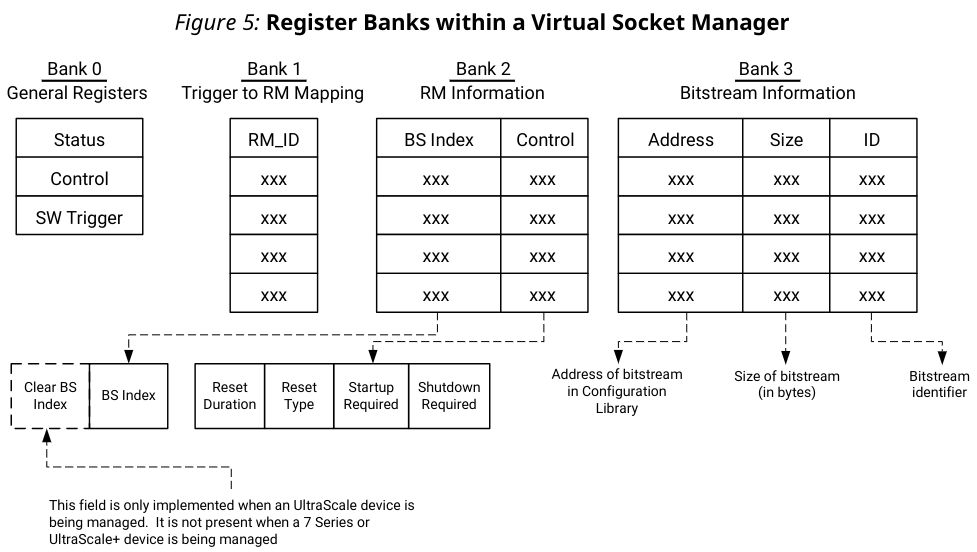
\includegraphics[width=0.65\textwidth]{images/dfx_ctrl_register.png}
\caption{\label{fig:dfx_ctrl} DFX Controller Architecture (copied from \cite{amd_dfx_controller_2026})}
\end{figure}

Fig.~\ref{fig:dfx_streamer} \cite{amd_dfx_controller_2026} illustrates the internal memory of the DFX CTRL IP. It is composed of 4 memory banks:

\begin{enumerate}
  \item Bank 0 contains general registers enabling software to control the IP and check its status.
  \item Bank 1 is the RM Mapping; each slot in this bank is a pointer to a slot in Bank 2.
  \item Bank 2 contains RM information. The control field is the setting of the start-up/shutdown procedure, and our driver sets these criteria as follows:
      \begin{enumerate}
        \item Reset Duration: 1 cycle
        \item Reset Type: active low
        \item Startup Required: No
        \item Shutdown Required: No
      \end{enumerate}
      The BS Index field contains the index of the target slot in Bank 3.
  \item Bank 3 contains the bitstream information:
      \begin{enumerate}
        \item Address: the address of the bitstream file in DDR memory
        \item Size: the size of the bitstream file in bytes
        \item ID: bitstream identifier
      \end{enumerate}
\end{enumerate}

In the case of multiple reconfigurable regions, the system will create Banks 0--3 equal to the number of the user's reconfigurable regions.

\subsection{DFX Decoupler Controller}

For debugging purposes, in the old version the DFX Controller IP owned the DFX decoupler, making it impossible for the PS to bypass control in some situations. We therefore redesigned the ownership of the DFX decoupler into a per-region mux (\texttt{dfx\_decup\_ctrl}), located at address \texttt{0xA001\_0000}. The register maps to the \texttt{decup\_and\_ctrl\_ps} port: bit~0 is the global source-select, and bits~\texttt{[N:1]} carry the per-region PS decoupler values (one bit per reconfigurable region, where $N = \text{NUM\_REGION}$). The resulting decoupler signal can be routed to \texttt{decup\_store}, \texttt{decup\_load}, or both on the target \texttt{Dfx\_Streamer}. The register bit-field definition is shown in Table~\ref{tab:dfx_decoupler_reg}.

\begin{table}[H]
  \centering
  \caption{DFX Decoupler Control Register (\texttt{0xA001\_0000}) bit-field definition.}
  \label{tab:dfx_decoupler_reg}
  \begin{tabular}{C{1.2cm} C{1.6cm} C{2.2cm} p{8.2cm}}
    \toprule
    \textbf{Bit} & \textbf{Access} & \textbf{Value} & \textbf{Description} \\
    \midrule
    \multirow{2}{*}{0} & \multirow{2}{*}{\badwo} &
        \texttt{1} & Decoupler source is the \textbf{DFX Controller} (used during partial reconfiguration). \\
    & & \texttt{0} & Decoupler source is the \textbf{PS} (used during debug/manual operation). \\
    \midrule
    \multirow{2}{*}{\texttt{r+1}} & \multirow{2}{*}{\badwo} &
        \texttt{1} & PS decoupler value for region~$r$ is \textbf{decoupled} (isolated). Valid only when Bit~0~\texttt{= 0} (PS source). \\
    & & \texttt{0} & PS decoupler value for region~$r$ is \textbf{coupled} (normal operation). Valid only when Bit~0~\texttt{= 0} (PS source). \\
    \bottomrule
  \end{tabular}
\end{table}



\subsection{Other Relevant IPs}

In DFX4ML, there are 3 other IPs that support system creation:
  \begin{enumerate}
    \item icapWrap is the module that serves as an interface for the DFX Controller to self-reconfigure. \textcolor{darkgreen}{\texttt{hw/ip\_src/dfx\_icap/dfx\_streamer.v}}
    \item Stream\_Master\_Dummy is the module used as a dummy plug on the partial region AXI-Stream master side. It is built to prevent unpredictable signals when the target reconfigurable module does not require certain interface ports. \newline\textcolor{darkgreen}{\texttt{hw/ip\_src/dfx\_streamer\_mshut/streamer\_mshut.v}}
    \item Stream\_Slave\_Dummy is similar to Stream\_Master\_Dummy but for the AXI-Stream slave side.\newline\textcolor{darkgreen}{\texttt{hw/ip\_src/dfx\_streamer\_sshut/streamer\_sshut.v}}
  \end{enumerate}


\section{Driver Architecture}


\paragraph{\textbf{Memory Address}}

Our build script sets a default base address of \addr{0xA000\_0000} for the DFX Unified IP, which includes DFX Mng IP, DFX Ctrl IP, DMA IP, PR Reset, and PR DECUP.

\begin{table}[h]
    \centering
    \caption{DFX Unified IP Address Map (Base: \addr{0xA000\_0000})}
    \label{tab:dfx_address_map}
    \begin{tabular}{lp{3.2cm}p{3.2cm}p{4.0cm}}
        \toprule
        \textbf{IP} & \textbf{Offset} & \textbf{Absolute \newline Address} & \textbf{Address Range} \\
        \midrule
        DFX Ctrl     & \addr{0x0\_0000} & \addr{0xA000\_0000} & \addr{0xA000\_0000} -- \addr{0xA000\_FFFF} \\
        PR DECUP     & \addr{0x1\_0000} & \addr{0xA001\_0000} & \addr{0xA001\_0000} -- \addr{0xA001\_FFFF} \\
        PR Reset     & \addr{0x2\_0000} & \addr{0xA002\_0000} & \addr{0xA002\_0000} -- \addr{0xA002\_FFFF} \\
        DMA          & \addr{0x3\_0000} & \addr{0xA003\_0000} & \addr{0xA003\_0000} -- \addr{0xA003\_FFFF} \\
        DFX Mng      & \addr{0x4\_0000} & \addr{0xA004\_0000} & \addr{0xA004\_0000} -- \addr{0xA004\_FFFF} \\
        PR Ctrl$^*$  & \addr{0x5\_0000} \newline $+\,r \times$ \addr{0x1\_0000}
                     & \addr{0xA005\_0000} \newline $+\,r \times$ \addr{0x1\_0000}
                     & \addr{0xA005\_0000} -- \addr{0xA005\_FFFF} \newline $+\,r \times$ \addr{0x1\_0000} \\
        \bottomrule
    \end{tabular}
    \\ \smallskip
    {\footnotesize $^*$ One instance per reconfigurable region; $r = 0, 1, \ldots, N{-}1$.}
\end{table}

\paragraph{\textbf{Driver Component}}

This section illustrates the PYNQ driver overview used to command the DFX4ML-ARCH hardware.

\begin{figure}[H]
\centering
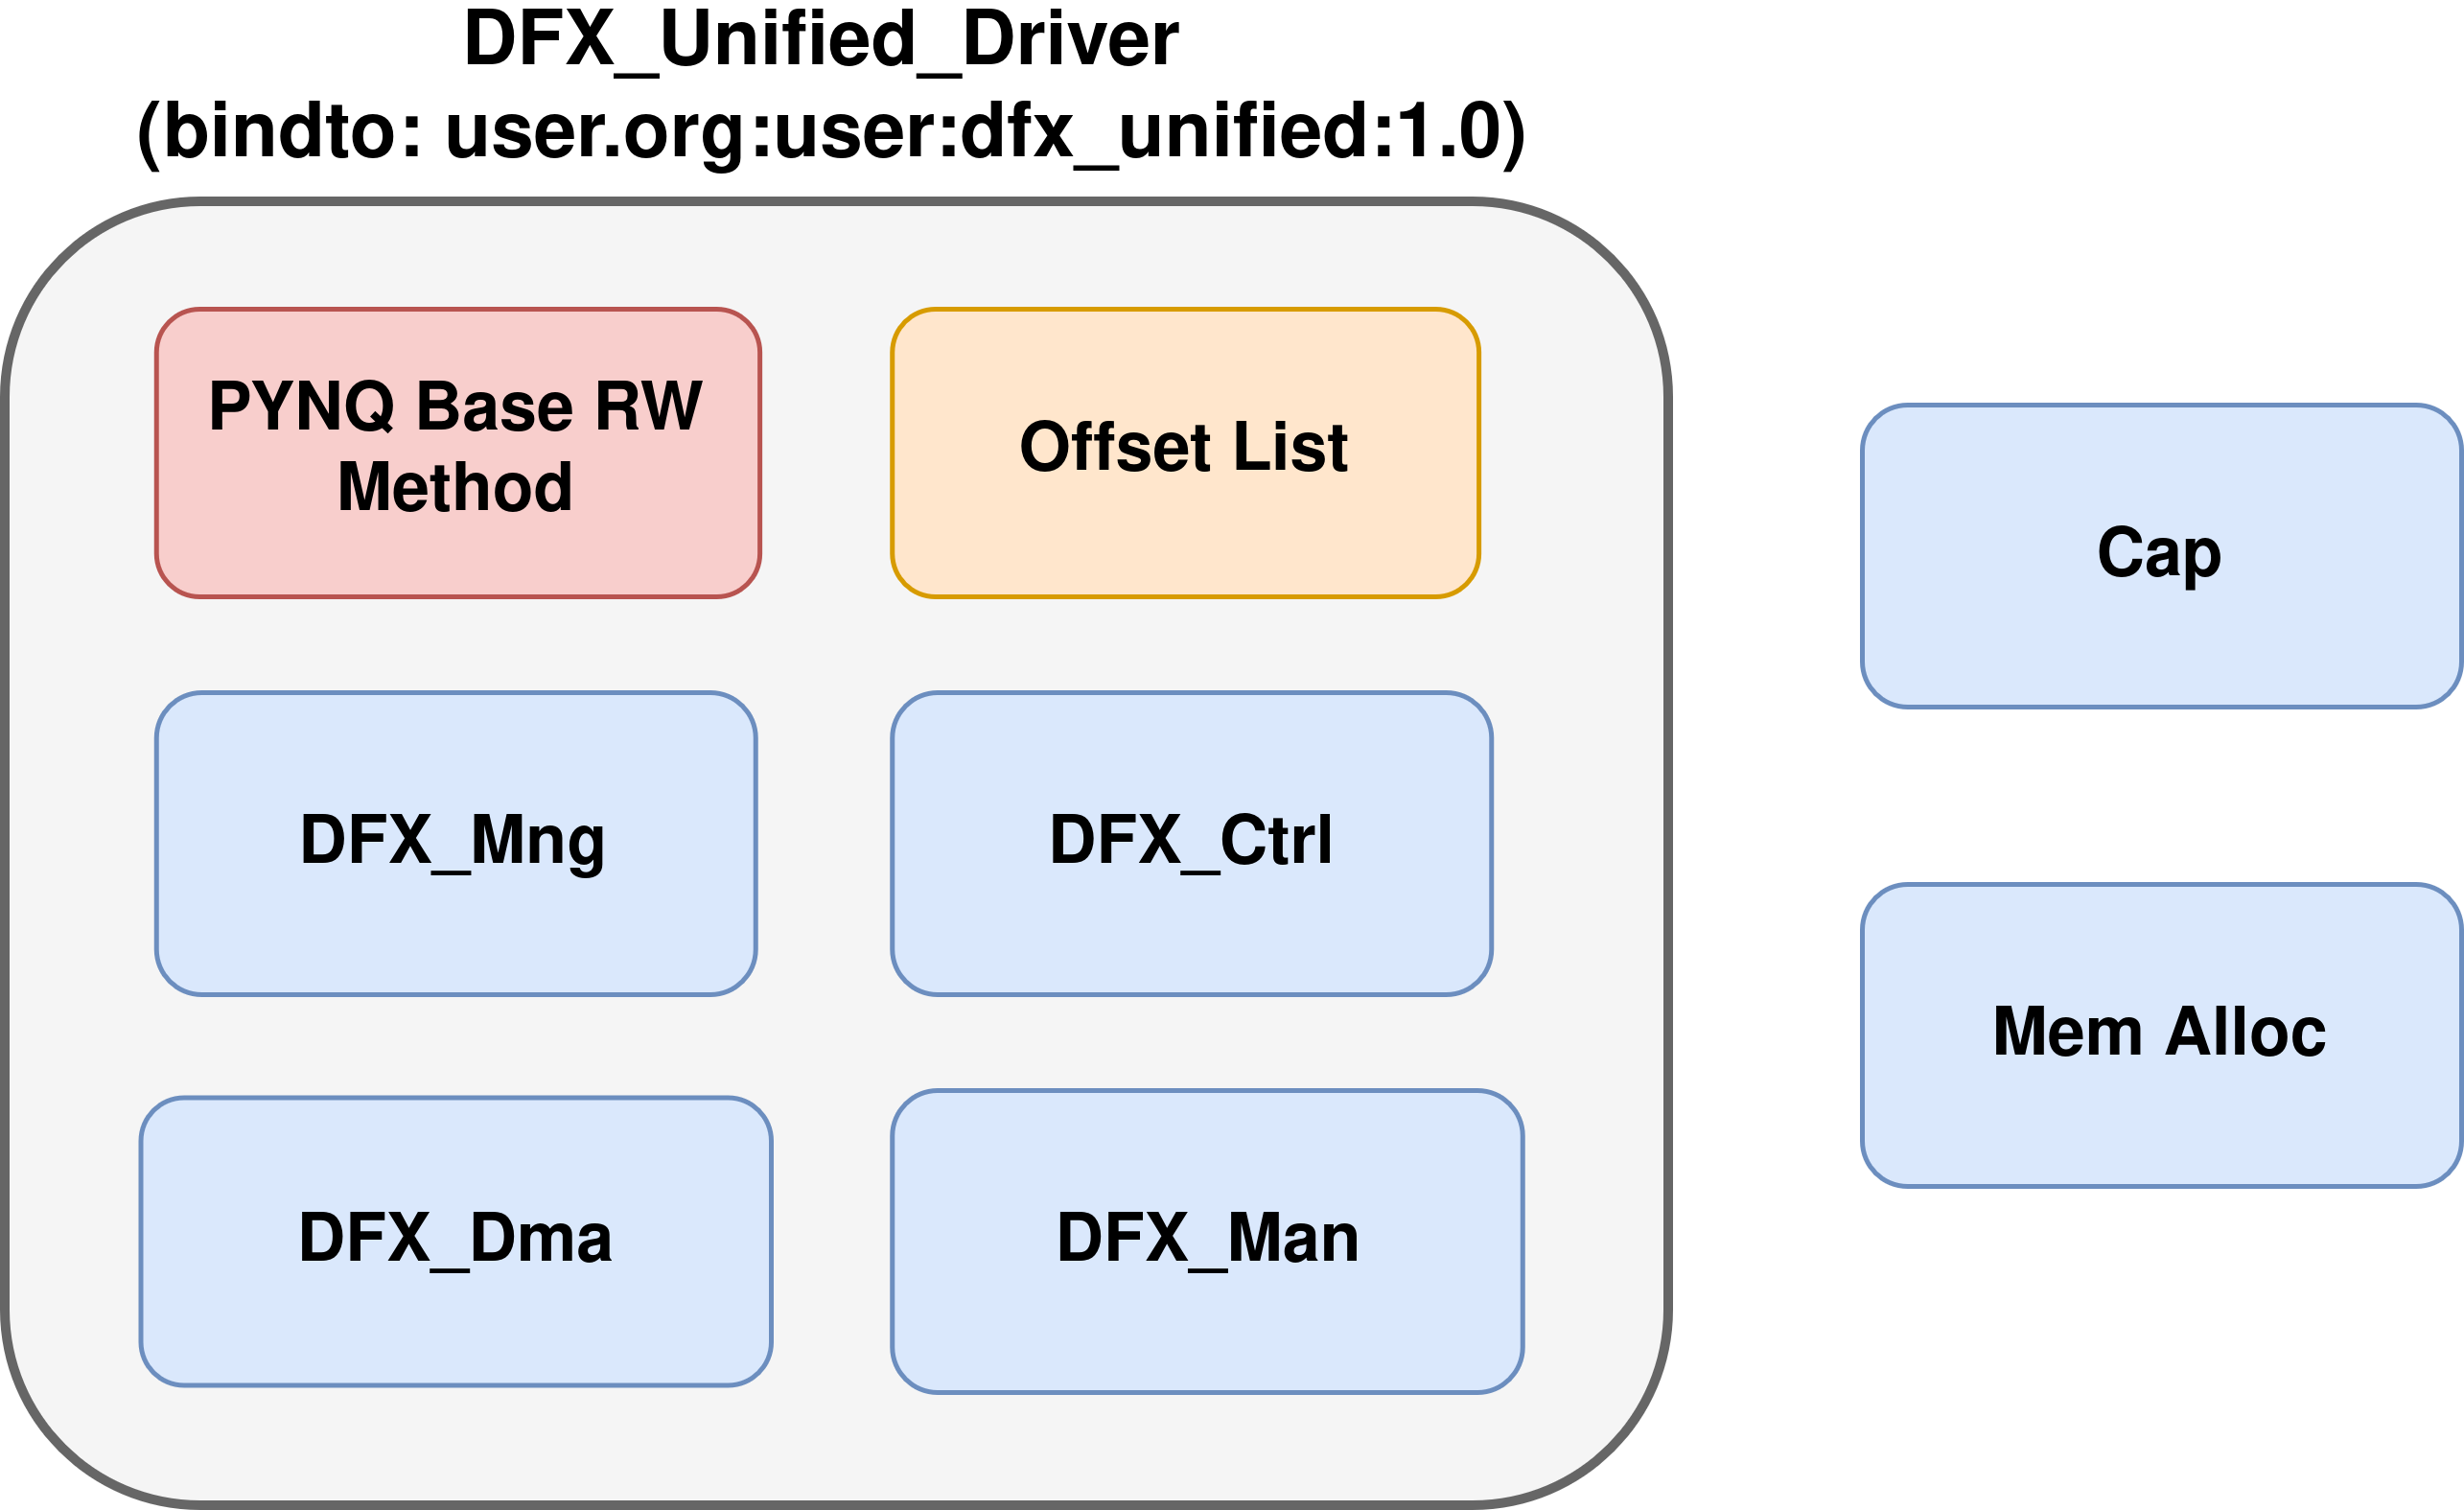
\includegraphics[width=0.65\textwidth]{images/software_diagram.png}
\caption{\label{fig:software_overview} DFX4ML-ARCH Driver Overview}
\end{figure}


\textbf{DFX\_Unified\_Driver}: This class controls the DFX Unified IP's operations. As described in the Hardware Architecture section, the DFX Unified IP is composed of 4 sub-IPs: DFX Manager, DFX Controller, DFX DMA, and DFX Streamer(s).

Therefore, \textbf{The Unified Driver} is composed of 4 sub-drivers (blue boxes): DFX Manager Driver to control the Reconfigurable Module's flow; DFX Controller Driver to manage the partial bitstream; DMA Driver to manage the memory data transfer, used for debugging purposes only; and DFX Manual, used to manually decouple and reset the partial region, also for debugging purposes only.

the code is at \newline
\textcolor{darkgreen}{\texttt{sw/driver/dfx\_unified.py}}\newline
\textcolor{darkgreen}{\texttt{sw/driver/dfx\_mng.py}}\newline
\textcolor{darkgreen}{\texttt{sw/driver/dfx\_ctrl.py}}\newline
\textcolor{darkgreen}{\texttt{sw/driver/dfx\_dma.py}}\newline
\textcolor{darkgreen}{\texttt{sw/driver/dfx\_man.py}}\newline


\textbf{Cap} is the helper function enabling designers to communicate with the PMU processor and reconfigure the \reg{pcap\_ctrl} register. After changing this register to 1, the FPGA will enable partial reconfiguration via the ICAP3 port. In contrast, if the register is set to 0, the FPGA will allow reconfiguration only from the processor (PS).

\textbf{Mem Alloc} is a helper function that facilitates users in allocating and copying data.


\pagebreak
\section{Build Procedure}


\subsection{Quick Start}

We provide a Python interface that allows users to generate full and partial bitstream files ($.bin$), hardware handoff files ($.hwh$), DFX Ctrl configuration files, and PYNQ driver files. 

\begin{lstlisting}[style=python, caption={Python Build Interface}, numbers=left, label={lst:python_build}]
from lib.hw_build import HwBuildHelper
from lib.sw_build import SwBuildHelper

# Streamer definitions (index 0 is always the DMA)
# load_width and store_width are in bytes
dfx_streamers = [
    {"load_width": 4, "store_width": 4, "actual_width": 32, "amount_row": 1024},
    {"load_width": 4, "store_width": 4, "actual_width": 32, "amount_row": 1024},
]

# Region definitions: two regions forming a pipeline DMA->r0->r1->DMA
dfx_regions = [
    {"load_streamers": [0], "store_streamers": [1]},
    {"load_streamers": [1], "store_streamers": [0]},
]

# RM schematics: rm_schemetics[region_idx][rm_idx]
# load_io_map/store_io_map: list of (streamer_index, kernel_port_index) pairs
rm_schemetics = [
    [{"load_io_map": [(0, 0)], "store_io_map": [(1, 0)]}],
    [{"load_io_map": [(1, 0)], "store_io_map": [(0, 0)]}],
]

# Hardware Build
hw_builder = HwBuildHelper(
    build_folder_path      = "./build_prj",
    dfx_root_path          = "../..",
    board                  = "custom",
    board_build_tcl        = "./kv260/board_build.tcl",
    constraint_xdc         = "./kv260/constraint.xdc",
    user_repo_path         = "",
    user_rm_build_tcl_path = "",
    req_gen_ip             = 1,
    num_core               = 4,
    clk_frq                = 99999001,
    rm_index_width         = 2,
    dfx_streamers          = dfx_streamers,
    dfx_regions            = dfx_regions,
    rm_schemetics          = rm_schemetics,
    test_mode              = 1,
    vivado_path            = "<vivado path>",
    export_folder_path     = "./export"
)
hw_builder.run_build()
hw_builder.package_export_files()

# Software Build
sw_builder = SwBuildHelper(
    export_folder_path = "./export",
    num_pr_region      = 2,
    rm_index_width     = 2,
    num_streamer       = 2
)
sw_builder.package_export_file()
\end{lstlisting}

The following example (Listing~\ref{lst:python_build}) demonstrates how to start building the DFX4ML-ARCH system. The reference file is at \textcolor{darkgreen}{\texttt{example/muti\_region\_test/multi\_region\_test.ipynb}}. Lines 1--2 import the Hardware and Software Build Helpers. Lines 6--22 define the three structured configuration objects (\texttt{dfx\_streamers}, \texttt{dfx\_regions}, \texttt{rm\_schemetics}). Lines 25--45 instantiate \texttt{HwBuildHelper} and invoke synthesis and implementation; Lines 48--54 instantiate \texttt{SwBuildHelper} and export the PYNQ driver files.

Table~\ref{tab:hw_build_params} describes each parameter of \texttt{HwBuildHelper}.

\renewcommand{\arraystretch}{1.3}
\begin{longtable}{|l|p{11cm}|}
\caption{HwBuildHelper Parameters}
\label{tab:hw_build_params} \\
\hline
\textbf{Parameter} & \textbf{Description} \\
\hline
\endfirsthead
\hline
\textbf{Parameter} & \textbf{Description} \\
\hline
\endhead
\hline
\endfoot
\texttt{build\_folder\_path} & Path to the directory where Vivado project files and other temporary working files are written. The folder will be created if it does not exist. \\
\hline
\texttt{dfx\_root\_path} & Root path of the DFX4ML-ARCH source repository, used to locate IP cores, build scripts, and constraint files. \\
\hline
\texttt{board} & Target FPGA board identifier. Use a known board name (e.g., \texttt{kv260}) or \texttt{"custom"} to supply \texttt{board\_build\_tcl} and \texttt{constraint\_xdc} manually. \\
\hline
\texttt{user\_repo\_path} & Path to the user-supplied IP repository containing partial-region kernels. Referenced only when \texttt{test\_mode=0}. \\
\hline
\texttt{user\_rm\_build\_tcl\_path} & Path to the user-supplied Tcl script that builds the reconfigurable module (RM) IP. Referenced only when \texttt{test\_mode=0}. \\
\hline
\texttt{req\_gen\_ip} & Flag (\texttt{1}/\texttt{0}) controlling whether Verilog IP generation is run before the build. The generated IPs are: ICAP interface, DFX Manager, DFX Streamer, and DFX Streamer Shut Plug. \textbf{Must be set to \texttt{1}} the first time or whenever \texttt{build\_folder\_path} has been deleted or modified. \\
\hline
\texttt{num\_core} & Number of parallel synthesis/implementation jobs to run in Vivado. \\
\hline
\texttt{clk\_frq} & Requested clock frequency in Hz (e.g., \texttt{99999001} $\approx$ 100\,MHz). \\
\hline
\texttt{rm\_index\_width} & Bit-width of the RM index field, which sets the number of slots in DFX Mng Bank\,1 and DFX Ctrl as $2^{\texttt{rm\_index\_width}}$ (e.g., \texttt{rm\_index\_width=2} allocates 4 slots). The actual number of loaded RMs is determined by \texttt{rm\_schemetics}. \\
\hline
\texttt{dfx\_streamers} & List of streamer configuration dicts, one per DFX Streamer instance. Index\,0 is always the DMA pass-through streamer. Each dict must contain: \texttt{load\_width} (bus width in bytes for load path, power of 2), \texttt{store\_width} (bus width in bytes for store path, power of 2), \texttt{actual\_width} (effective data width in bits, $\leq$ bus width $\times$ 8), and \texttt{amount\_row} (internal BRAM depth in rows). \\
\hline
\texttt{dfx\_regions} & List of region configuration dicts, one per reconfigurable region. Each dict must contain: \texttt{load\_streamers} (list of streamer indices that supply data to this region) and \texttt{store\_streamers} (list of streamer indices that receive data from this region). Indices must be valid entries in \texttt{dfx\_streamers}. \\
\hline
\texttt{rm\_schemetics} & Two-dimensional list of RM schematic dicts indexed as \texttt{rm\_schemetics[region\_idx][rm\_idx]}. Each dict must contain: \texttt{load\_io\_map} (list of \texttt{(streamer\_index, kernel\_port\_index)} pairs for input connections) and \texttt{store\_io\_map} (list of \texttt{(streamer\_index, kernel\_port\_index)} pairs for output connections). All regions must declare the same number of RMs. \\
\hline
\texttt{test\_mode} & Flag (\texttt{1}/\texttt{0}) enabling test mode. When set, loopback logic is inserted for hardware verification without a user RM. Set to \texttt{0} to use the actual user kernel. \\
\hline
\texttt{vivado\_path} & Absolute path to the Vivado executable (e.g., \texttt{"/tools/Xilinx/Vivado/2023.2/bin/vivado"}). \\
\hline
\texttt{export\_folder\_path} & Destination directory for packaged output files (\texttt{.bin}, \texttt{.hwh}, DFX Ctrl configuration, and PYNQ drivers). The folder will be created if it does not exist. \\
\hline
\texttt{board\_build\_tcl} & \textit{(Optional; required when \texttt{board="custom"})} Path to the board-specific Tcl build script. Ignored for known board identifiers. \\
\hline
\texttt{constraint\_xdc} & \textit{(Optional; required when \texttt{board="custom"})} Path to the board-specific XDC constraint file. Ignored for known board identifiers. \\
\hline
\end{longtable}
 


\subsection{ML Framework Integration}

DFX4ML-ARCH provides the official solution for enabling Hardware Machine Learning frameworks to integrate their own sub-kernels into each Reconfigurable Module (RM).

To integrate the module, users must complete the following steps:
\begin{enumerate}
    \item Provide the path to the user IP repository via \texttt{user\_repo\_path}. The folder at that path must contain the Vivado-exported IP folder, which in turn must include \texttt{src} and \texttt{xgui} sub-folders.
    \item Provide the path to the TCL file that instructs the build script how to build the Reconfigurable Module via \texttt{user\_build\_tcl} (Listing~\ref{lst:python_build}).
    \item Set \texttt{test\_mode} to \texttt{0} (Listing~\ref{lst:python_build}) to enable the actual kernel instead of the loopback test logic.
    \item Provide the IP name list in $ip\_map\_list$ (Listing~\ref{lst:python_build}). The index corresponds to the Reconfigurable Module and the value is the IP name.
\end{enumerate}


\subsubsection{User Build Tcl}

The user build TCL file must define the \texttt{create\_dfx\_region\_bd} procedure with the following signature:

\begin{lstlisting}[style=tcl, caption={User Build TCL Procedure Signature}, label={lst:user_build_tcl}, numbers=left]
proc create_dfx_region_bd { \
    parentCell \
    block_name \
    clk_frq \
    interface_widths \
    rm_config \
    ip_name \
    rm_id \
} {
    # User implementation here
}
\end{lstlisting}

Table~\ref{tab:tcl_params} describes each argument of the procedure.

\begin{longtable}{|l|p{11cm}|}
\caption{create\_dfx\_region\_bd Arguments}
\label{tab:tcl_params} \\
\hline
\textbf{Argument} & \textbf{Description} \\
\hline
\endfirsthead
\hline
\textbf{Argument} & \textbf{Description} \\
\hline
\endhead
\hline
\endfoot
\texttt{parentCell} & This field is deprecated. \\
\hline
\texttt{block\_name} & Name of the hierarchical block representing the Reconfigurable Module in the block design. \\
\hline
\texttt{clk\_frq} & Clock frequency in Hz passed from \texttt{HwBuildHelper}, used to configure IP timing constraints inside the region. \\
\hline
\texttt{interface\_widths} & List of data-bus widths (bits) for each DFX Streamer, derived from \texttt{dfx\_streamers} in \texttt{HwBuildHelper}. Each entry is the bus width in bits for the corresponding streamer index. \\
\hline
\texttt{rm\_config} & RM schematic dict for this specific (region, RM) pair, corresponding to one element of \texttt{rm\_schemetics} in \texttt{HwBuildHelper}. Must contain two keys: \texttt{load\_io\_map} (list of \texttt{\{streamer\_index kernel\_port\_index\}} pairs for input connections) and \texttt{store\_io\_map} (list of \texttt{\{streamer\_index kernel\_port\_index\}} pairs for output connections). \\
\hline
\texttt{ip\_name} & IP core name string for this kernel slot. An empty string indicates no additional IP is mapped. \\
\hline
\texttt{rm\_id} & Zero-based integer identifier of the Reconfigurable Module within its region, used to uniquely name generated block design elements. \\
\hline
\end{longtable}


The argument \texttt{rm\_config} is passed directly from the corresponding element of \texttt{rm\_schemetics} defined in \texttt{HwBuildHelper} (Listing~\ref{lst:python_build}).

Users must provide the RM implementation, which includes:

\begin{enumerate}
  \item Create Block Design
  \item Add ML IP module
  \item Connect the I/O (clk, nreset (active low), AXI-Stream interface(s))
  \item Validate Block Design
  \item Close Block Design
\end{enumerate}

Users may use \textcolor{darkgreen}{\texttt{hw/bd\_src/dfx\_region/dfx\_region.tcl}} as a reference.


\subsection{Board-Specific Script}

In the current version, only the KV260 board can be fully synthesized and implemented. If the $board$ parameter is set to $custom$, the hardware build will stop at the DFX block design with DFX Unified and partial connections; the PS and interconnect will be missing.

To define a new board, users must create or modify the following files:
  \begin{enumerate}
    \item \texttt{board\_file}: users must create the file at \newline\textcolor{darkgreen}{\texttt{hw/build\_script/<your board name>/board\_build.tcl}} \newline The purpose of this file is to provide a processor block, interconnect block, interrupt system, and other relevant IPs in the Vivado block design. Users can use \newline\textcolor{darkgreen}{\texttt{hw/build\_script/kv260/board\_build.tcl}} or the GUI in board $custom$ as a reference.
    \item \texttt{constraint\_file}: users must create one file per supported region count at \newline\textcolor{darkgreen}{\texttt{hw/build\_script/<your board name>/constraint\_<N>\_region.xdc}} \newline where \texttt{<N>} is the number of reconfigurable regions; the build selects the file matching \texttt{num\_dfx\_region}. The purpose of these files is to define the boundaries of each partial reconfigurable region and its resources. Users can use \newline\textcolor{darkgreen}{\texttt{hw/build\_script/kv260/constraint\_1\_region.xdc}} and \newline\textcolor{darkgreen}{\texttt{hw/build\_script/kv260/constraint\_2\_region.xdc}} as references (the KV260 currently supports 1 and 2 regions).
    \item \texttt{build\_script}: users must modify the file at \newline\textcolor{darkgreen}{\texttt{hw/build\_script/build.tcl}} to invoke the block design creation procedure. Users may use the kv260 option as a reference.
  \end{enumerate}

The DFX4ML-ARCH authors would appreciate pull requests for board-specific files.

\bibliography{references}
\bibliographystyle{plain}

\end{document}